\documentclass[a4paper, 11pt]{article}

\usepackage[utf8]{inputenc}
\usepackage[T1]{fontenc}
\usepackage[francais]{babel} 
\usepackage{amsmath} % pour les formules de maths
\usepackage{amssymb} % pour des symboles
\usepackage{mathrsfs} % pour avoir acces a des jolies lettres calligrafiées.:)
\usepackage{listings} % pour le code source
\usepackage{color} % pour les couleurs
\usepackage{graphicx} % pour les graphiques (images)
\usepackage{fancyhdr} % pour utiliser le pagestyle fancy
\usepackage[headheight=10pt]{geometry} % pour les marges
\usepackage[T1,hyphens]{url}
\usepackage{float}
\usepackage{titlesec}
\usepackage{cite}
\usepackage{rotating}
\usepackage[colorinlistoftodos,prependcaption,textsize=tiny]{todonotes}

\usepackage[perpage, bottom]{footmisc}
\usepackage[colorlinks,urlcolor=blue, linkcolor=blue]{hyperref}
\usepackage[colorlinks,urlcolor=blue, linkcolor=blue]{hyperref}


%%%%%%%%%%%%%%%%%%%%%%%%%%%
% define subsubsubsection %
%%%%%%%%%%%%%%%%%%%%%%%%%%%

\titleclass{\subsubsubsection}{straight}[\subsection]

\newcounter{subsubsubsection}[subsubsection]
\renewcommand\thesubsubsubsection{\thesubsubsection.\arabic{subsubsubsection}}
\renewcommand\theparagraph{\thesubsubsubsection.\arabic{paragraph}} % optional; useful if paragraphs are to be numbered

\titleformat{\subsubsubsection}
  {\normalfont\normalsize\bfseries}{\thesubsubsubsection}{1em}{}
\titlespacing*{\subsubsubsection}
{0pt}{3.25ex plus 1ex minus .2ex}{1.5ex plus .2ex}

\makeatletter
\renewcommand\paragraph{\@startsection{paragraph}{5}{\z@}%
  {3.25ex \@plus1ex \@minus.2ex}%
  {-1em}%
  {\normalfont\normalsize\bfseries}}
\renewcommand\subparagraph{\@startsection{subparagraph}{6}{\parindent}%
  {3.25ex \@plus1ex \@minus .2ex}%
  {-1em}%
  {\normalfont\normalsize\bfseries}}
\def\toclevel@subsubsubsection{4}
\def\toclevel@paragraph{5}
\def\toclevel@paragraph{6}
\def\l@subsubsubsection{\@dottedtocline{4}{7em}{4em}}
\def\l@paragraph{\@dottedtocline{5}{10em}{5em}}
\def\l@subparagraph{\@dottedtocline{6}{14em}{6em}}
\makeatother

\setcounter{secnumdepth}{4}
\setcounter{tocdepth}{4}

%%%%%%%%%%%%%%%%%%%%%%%%
% end subsubsubsection %
%%%%%%%%%%%%%%%%%%%%%%%%

%%%%%%%%%%%%%%
% start code %
%%%%%%%%%%%%%%
\definecolor{green}{rgb}{0.0, 1.0, 0.0}
\definecolor{purple}{rgb}{0.62, 0.0, 0.77}
\lstdefinestyle{customc}{
  belowcaptionskip=1\baselineskip,
  breaklines=true,
  frame=L,
  xleftmargin=\parindent,
  language=Java,
  showstringspaces=false,
  basicstyle=\footnotesize\ttfamily,
  keywordstyle=\bfseries\color{green},
  commentstyle=\itshape\color{purple},
  identifierstyle=\color{blue},
  stringstyle=\color{orange},
}

\lstdefinestyle{customasm}{
  belowcaptionskip=1\baselineskip,
  frame=L,
  xleftmargin=\parindent,
  language=[x86masm]Assembler,
  basicstyle=\footnotesize\ttfamily,
  commentstyle=\itshape\color{purple},
}

\lstset{escapechar=@,style=customc}

%%%%%%%%%%%%
% end code %
%%%%%%%%%%%%

\geometry{hmargin=3cm}

\title{Projet de Master}
\author{Romain Mencattini}
\date{\today}

\pagestyle{fancy} % pour avoir des entetes et des pieds de page
\renewcommand\headrulewidth{0.6pt}
\fancyhead[L]{Romain Mencattini} % haut de page gauche
\fancyhead[R]{Université de Genève \today} % haut de page droite

\begin{document}
\maketitle
\newpage
\tableofcontents
\newpage

%%%%%%%%%%%%%%%%%%%%%%%%%%%%%%%%%%%%%%%%%%%%%%%%%%%%%%%%%%%%%%%%%%%%%%%%%%
% début l'introduction     %%%%%%%%%%%%%%%%%%%%%%%%%%%%%%%%%%%%%%%%%%%%%%%
%%%%%%%%%%%%%%%%%%%%%%%%%%%%%%%%%%%%%%%%%%%%%%%%%%%%%%%%%%%%%%%%%%%%%%%%%%
\section{Introduction}
\paragraph{}
Ces dernières années, avec l'augmentation de la puissance de calcul et des données à dispositions, l'intelligence artificielle et son sous-domaine le \textit{machine learning} ont connu une forte croissance. Que ce soit avec la victoire d'une machine face à un humain au jeu de Go \cite{deepmind}, ou bien lorsque des programme de Microsoft et Alibab sont capable de mieux lire qu'un être humain \cite{microsoft_reading}, les progrès permettent de dépasser les humains dans des tâches dont on n'imaginait difficilement qu'elles puissent être réalisées par des machines.

\paragraph{}
De nombreux domaines comme les jeux, la linguistique, l'imagerie sont concernés. C'est également, dans une certaine mesure, le cas pour la finance.
C'est l'intersection de ces deux domaines, l'intelligence artificielle et la finance, que nous allons étudier dans un premier temps, afin d'introduire et de développer une application d'apprentissage automatique qui officiera sur le marché des changes.
Le document se décomposera en deux grandes axes. 

\paragraph{}
La première partie consiste en un état de l'art. Ce dernier nous permettra d'aborder et de définir le marché des changes ainsi que les concepts et formules mathématiques derrières plusieurs techniques d'apprentissage. Nous aborderont un certain nombres d'algorithmes qui comprendra la descente du gradient, les réseaux de neurones, la régression logistique ou les arbres de décisions. Cela nous permettra d'avoir un large horizon de techniques et d'options en vue de réaliser un apprentissage automatique. Une fois ces deux éléments expliqués, nous combinerons ces deux domaines pour montrer les applications possibles ainsi que les pistes de réflexions. Ceci conclura notre état de l'art.

\paragraph{}
La seconde se focalisera sur le projet en lui-même. Nous présenterons de manière précise et détaillée l'algorithme sur lequel se base notre recherche. Il y sera également question de l'implémentation, soit comment la formulation mathématique a été traduite en code informatique. Nous traiterons également des points problématiques ainsi que des remédiations possibles. Après une analyse des résultats de l'algorithme, nous conclurons le document et nous proposerons plusieurs pistes pour des recherches futures.


%%%%%%%%%%%%%%%%%%%%%%%%%%%%%%%%%%%%%%%%%%%%%%%%%%%%%%%%%%%%%%%%%%%%%%%%%%
% début de l'état de l'art %%%%%%%%%%%%%%%%%%%%%%%%%%%%%%%%%%%%%%%%%%%%%%%
%%%%%%%%%%%%%%%%%%%%%%%%%%%%%%%%%%%%%%%%%%%%%%%%%%%%%%%%%%%%%%%%%%%%%%%%%%
\section{État de l'art}
\subsection{Introduction}
\paragraph{}
Avant la démocratisation de l'informatique, les opérations financières étaient réalisées par des humains. 
Ce système pouvait avoir des inconvénients:
\begin{itemize}
\item L'émotionnel influençait les transactions. En effet, ces dernières étant effectuées par des humains, 
il y avait un risque non négligeable que l'état de la personne agisse sur sa décision.

\item Un problème sous-jacent était de maintenir une discipline de \textit{trading}. 
Afin de minimiser les pertes et de maximiser les gains, il fallait se tenir à un plan afin de ne pas se laisser 
influencer par des paramètres extérieurs. Cela pouvait être très difficile.

\item Le \textit{backtesting}\footnote{Le \textit{Backtesting} est le processus qui consiste à tester une stratégie
de \textit{trading} sur des données historiques afin de s'assurer de sa viabilité avant de risquer du capital.
\cite{investopedia_backtesting}} 
était impossible. Tester la qualification ainsi que la qualité de \textit{trading} d'une personne était compliquée. 
De même pour un \textit{trading plan}.
\end{itemize}

\paragraph{}
Ces éléments ont, en partie, favorisé l'émergence et l'utilisation d'algorithmes dans la finance. 
En 2014 aux États-Unis, 84\% des transactions étaient accomplies par des algorithmes \cite{real_investors}. 
Ce qui représente environ 100'000 réalisations, ou \textit{ticks}, par secondes \cite{real_investors}. L'informatique a engendré une automatisation très importante des transactions.
Durant l'évolution de l'outil informatique, le monde de la finance en a suivi les améliorations afin de perfectionner 
leurs algorithmes. L'automatisation mise à part, on retrouve des méthodes d'optimisations poussées ainsi que les récentes découvertes 
de \textit{data mining} et de \textit{machine learning}, abrégé \textit{ML}. 
Des propositions de plus en plus pointues dans les deux domaines voient le jour. 
L'algorithme qui sera au cœur de ce projet en fait partie. 
Il s'agit d'un réseau de neurones avec plusieurs couches prenant en compte des paramètres particuliers à la finance.

\paragraph{}Afin d'approcher aux mieux ces notions, nous allons discuter des éléments nécessaires à leur compréhension.
Nous allons en premier lieu traiter le domaine financier ainsi que ces outils. Puis nous parlerons de 
plusieurs méthodes de \textit{ML}. Il est compliqué d'être exhaustif tant les méthodes sont nombreuses et disposent de variations complexes. Les algorithmes choisis présenterons un large panel de techniques et constitueront une introduction complète au domaine. Ces derniers comprendront les réseaux de neurones, les arbres de décision, le \textit{Support Vector Machine}\cite{wikipedia_svm}, les classifieurs \textit{Naive Bayes} ainsi que la descente du gradient \cite{wikipedia_descente_du_gradient} et sa version dite stochastique \cite{descente_du_gradient_stochastique}.


Finalement, nous lierons les deux domaines en montrant comment adapter les modèles mathématiques de \textit{ML} pour les utiliser comme techniques de \textit{trading}, en évaluant leur performances.


\subsection{Finance}

\subsubsection{\textit{FOREX}}

\paragraph{}
Avant de parler du \textit{FOREX}, il convient d'en donner une définition \cite{forex_definition} :
\begin{center}
	"\textit{Forex (FX) is the market in which currencies are traded. The forex market is the largest, most liquid market in the world [...]. It includes all of the currencies in the world. There is no central marketplace for currency exchange; trade is conducted over the counter. The forex market is open 24 hours a day, five days a week, except for holidays, and currencies are traded worldwide among the major financial centers of London, New York, Tokyo, Zürich, Frankfurt, Hong Kong, Singapore, Paris and Sydney.[...] any person, firm or country may participate in this market.}"
\end{center}
Ce marché permet de faire des transactions sur toutes les monnaies. Il n'y a pas de place centrale, les échanges pouvant être conduits par les pays. Précision importante, chaque personne peut participer au \textit{FOREX}.

Afin d'appréhender le fonctionnement du \textit{FOREX}, il est important de mentionner certaines décisions historiques. Ces dernières ayant façonné le marché des devises actuel.

\paragraph{}
Jusqu'à la première guerre mondiale, le système en vigueur se basait sur l'or, que l'on nommait l'étalon-or\footnote{Source: \cite{etalon_or_a_etalon_dollar}.}. S'en suit une période d'instabilité notamment dûe aux pertes occasionnées par la guerre, un après-guerre compliqué, la crise boursière de 1929 et la seconde guerre mondiale.

C'est au sortir de cette dernière, que la nécessité de "\textit{mettre en place une organisation monétaire mondiale et de favoriser la reconstruction et le
développement économique des pays touchés par la guerre}" \cite{wikipedia_bretten_woods}, est apparue.
Le but était également "\textit{d’aplanir les conflits économiques, reconnaissant par là les problèmes engendrés par les disparités économiques}"
\cite{etalon_or_a_etalon_dollar}.

Plusieurs idées furent proposées, mais ce fût celle de Harry Dexter White qui fût mise en place. Cette dernière prévoyait entre autre:
\begin{itemize}
\item le choix du Dollar américain comme étalon, avec rattachement à l'or\footnote{Suspension de l'équivalence or pour le dollar américain en août 1971 puis abandon 
définitif en mars 1973 \cite{wikipedia_bretten_woods}.}.
\item Création de la Banque internationale pour la reconstruction et le développement (BIRD) qui deviendra la banque mondiale.
\item Le Fond monétaire international (FMI).
\item Création de l'Organisation mondiale du commerce\footnote{Ne verra le jour qu'en 1995 faute d'accord \cite{wikipedia_bretten_woods}.}.
\end{itemize}

On remarque que ces institutions sont toujours en activités, 
cela démontre l'importance de ces accords pour le système financier actuel.

\paragraph{}
Le marché \textit{FOREX} porte sur les devises. La valeur d'une devise ne peut être exprimée qu'en fonction d'une autre. 
Par exemple 1 franc suisse vaut 1.05 euro.\footnote{Taux fictif utilisé pour l'exemple.}
La transaction porte donc sur deux monnaies comme CHF/EUR. On va vendre des francs suisses pour acheter des euros ou l'inverse.
Le nom du marché vient d'ailleurs de ces échanges. 
On échange une monnaie contre une autre, c'est un \textit{FOreign EXchange}, ou \textit{FOREX}.

Il y a deux variations possibles:
\begin{itemize}
\item La monnaie peut subir une dépréciation.
\item La monnaie peut subir une appréciation.
\end{itemize}
Lorsque le prix d'une devise augmente par rapport à une monnaie étrangère, on parle d'appréciation. 
Ainsi dans le cas contraire, on parlera d'une dépréciation.

La mondialisation a facilité ce marché. En effet, toutes devises étant accessibles depuis 
n'importe où, il devient donc possible d'avoir des marchés avec des devises plus exotiques.
Il devient par exemple possible de vendre une monnaie avec un faible taux d'intérêt puis utiliser les fonds générés par la vente pour investir dans une monnaie avec un meilleur taux d'intérêt. Le but étant de capturer le différentiel d'intérêt \cite{currency_carry_trade}.

\paragraph{}
Les principaux acteurs financiers sont \cite{marche_des_changes}:
\begin{itemize}
\item Les banques commerciales. 
Elles peuvent pratiquer des interventions directes car elles gèrent des dépôts et veulent opérer des transactions sur ces derniers.
Il leur est également possible de réaliser le rôle d'intermédiaire financier.

\item Les entreprises. Ces dernières vont pratiquer des transactions directes, si elles disposent d'un accès aux marchés
sinon via des intermédiaires.

\item Les institutions financières non-bancaires. On peut citer les fonds de pensions, les sociétés d'assurances
ou les \textit{hedge funds}. Ce sont surtout dans un but de spéculation, d'arbitrage ou de couverture de risque qu'elles agissent.

\item Les banques centrales. Il peut y avoir des interventions directes, dans le but de modifier l'appréciation de la monnaie.

\item Les ménages. Surtout dans une optique de voyage, d'achat ou de spéculation.
\end{itemize}

\paragraph{}
Henry Bourguinat a énoncé "\textit{la règle des trois unités}" qui correspondent aux unités de temps, de lieu 
et d'opérations et d'acteurs.
Le \textit{FOREX} répond à ces trois unités \cite{site_fr_forex}:
\begin{itemize}
\item Ce marché fonctionne 24h/24 et les transactions s'effectuent presque en continue.

\item Il fonctionne à l'échelle mondiale tout en étant décentralisé. 
De part l'évolution des technologies, l'information circule aisément malgré son statut.

\item L'uniformité des procédés ainsi que des produits est présente. Les acteurs malgré nationalité sont de même nature.
\end{itemize}

\paragraph{}
Il existe principalement deux horizons temporels: le \textit{spot} et le \textit{forward}.

Le premier est également appelé "Le marché au comptant". Lorsque deux acteurs se mettent d'accord sur une transaction,
cette dernière se réalise 
immédiatement\footnote{Valable en théorie, dans la réalité cela peut prendre du temps \cite{marche_des_changes}}.

Le second peut être nommé "Le marché à terme". L'accord est passé à un temps $T$ mais la transaction effective ne
se réalise que dans le futur. Il également possible que la transaction ne se réalise pas. Ce futur, ou maturité, peut être de plusieurs dizaines de jours,
voir des années, soit $T + X$\footnote{Où $T$ est le moment présent, et $X$ une durée de temps.}.

Il y a des opérations réalisable sur le marché à terme :
\begin{itemize}
\item Les \textit{swaps}. Ils consistent à vendre une monnaie au comptant puis à la racheter à terme\footnote{Soit à $T+X$}.

\item Les \textit{futures/forwards}. La différence entre ces deux tient surtout à leur standardisation et leur mise en place.
Cependant le principe reste le même: on réalise une opération (d'achat ou de vente) qui ne s'effectuera qu'à maturité.

\item Les \textit{options}. Cela représente un contrat vendu par un parti (\textit{the option writer}) 
à un autre parti (\textit{the option holder}). Ce contrat offre le droit, et non l'obligation contrairement 
aux \textit{futures/forwards}, d'acheter (\textit{call}) ou de vendre (\textit{put}). Ici encore, il faut attendre la maturité
\footnote{Cela est vrai pour les options dites européennes\cite{investopedia_option_europeenne}. 
Dans le cas des options américaines\cite{investopedia_option_americaine}, le droit peut s'exercer à n'importe quel moment, offrant
ainsi une plus grande flexibilité.}.
\end{itemize}

Les options sont très versatiles. Elles peuvent être utilisées afin de spéculer ou de diminuer le risque. Voici les différents types possibles:
\begin{itemize}
\item \textbf{long call} $\rightarrow$ on achète le droit d'acheter le sous-jacent à un certain prix.
\item \textbf{short call} $\rightarrow$ on vend le droit d'acheter le sous-jacent à un certain prix.
\item \textbf{long put} $\rightarrow$ on achète le droit de vendre le sous-jacent à un certain prix.
\item \textbf{short put} $\rightarrow$ on vend le droit de vendre le sous-jacent à un certain prix.
\end{itemize}

\paragraph{}
Le \textit{bid} est le prix maximum qu'un acheteur est d'accord de payer pour un sous-jacent.
De la même manière, le \textit{ask} est le prix minimum qu'un vendeur accepte pour vendre 
un sous-jacent \cite{investopedia_bid_ask}.

La différence entre le \textit{bid} et le \textit{ask}, appelée le \textit{spread}, représente la liquidité d'un actif. 
Il est également utilisé comme marge par les \textit{broker}\cite{wikipedia_broker} et autres plateformes.



\subsection{Cadre théorique des algorithmes de \textit{Machine Learning}}
\subsubsection{Introduction}
\paragraph{}
T. Mitchell a donné une définition formelle \cite{mitchell}:
\begin{center}
"\textit{A computer program is said to learn from experience $E$ with respect to some class of tasks $T$ and
performance measure $P$ if its performance at tasks in $T$, as measured by $P$, improves with experience $E$}"
\end{center}

Cette citation signifie que si nous disposons d'une tâche $T$ à accomplir. $T$ peut consister à trier des images ou à reconnaître des motifs.
La mesure de la réussite de $T$ est nommée $P$. C'est-à-dire la qualité du résultat pour 
la tâche donnée, $T$. Si le programme améliore $P$ pour la tâche $T$ grâce à l'expérience $E$. 
Il s'agit d'un programme de \textit{machine learning}. L'expérience $E$ peut être vue comme une phase d'entraînement
ou comme le fait de retenir les réponses après avoir accompli la tâche.

\paragraph{}
Il existe deux catégories d'apprentissage:
\begin{itemize}
\item L'apprentissage supervisé.
\item L'apprentissage non-supervisé.
\end{itemize}

Dans le cas du premier, on fournit au programme, un ensemble d'entraînement\footnote{Ou d'expérience, $E$},
qui contient des réalisations ainsi que le résultat de la classification. 
Le programme va donc pouvoir utiliser ce savoir afin d'améliorer sa performance $P$.
Nous disposons donc de nombreux couples $(x_i, y_i)$ et le but est de trouver une fonction $f \in F$ telle que: $f(x) = y$.

Pour l'apprentissage non-supervisé, on fournit des données, mais sans le résultat voulu.
C'est uniquement après avoir décidé d'une valeur qu'on va signifier au programme si cette dernière est correcte.
On ne lui donnera jamais la valeur attendue. Il va donc utiliser uniquement les résultats précédents pour améliorer son $P$.

Par exemple, on désire reconnaître un certain type de voiture à partir d'images. Dans le cas de l'apprentissage supervisé,
nous allons fournir au programme un ensemble d'entraînement qui contient de nombreuses photos de voitures,
ainsi que la marque des dites voitures. L'algorithme va donc travailler avec ces données.

Par contre dans le cas de l'apprentissage non-supervisé, le programme ne pourra utiliser que les photos,
et après avoir retourné le résultat, nous lui dirons si c'est juste ou faux. Il mémorisera le résultat 
optimisera en conséquence ses réponses.

\paragraph{}
Concernant, l'ensemble d'entraînement, il y a des points à prendre en compte afin de minimiser les risques de sur-apprentissage\footnote{Le sur-apprentissage consiste à apprendre par cœur la tâche, plutôt que d'apprendre les principes pour réaliser la tâche.}, et de maximiser la qualité de nos données.
Pour ce faire il faut:\label{astuce ensemble d'entraînement}
\begin{itemize}
\item Représenter la population générale. Donc si le but est du traitement de la langue, 
il faut que la propension et la répartition des mots soient les mêmes que ceux de la langue.

\item Contenir des membres de chacune des classes. Pour reconnaître des chiffres, il est important de disposer de chacun 
des chiffres dans l'ensemble d'entraînement.
\item Contenir de grandes variations ainsi que du bruit. Afin d'éviter le sur-apprentissage, 
il faut de nombreux exemples différents, voir très différents, les uns des autres ainsi que 
du bruit\footnote{Comme des faux exemples.}.
\end{itemize}

\paragraph{}
Il est important de saisir comment fonctionne les algorithmes de \textit{machine learning}. 
Le but est d'utiliser des données, souvent de très hautes dimensionnalités\footnote{Cela signifie qu'elles 
sont représentées par un grand nombre d'attributs.}, dans des équations dont on pourra faire varier 
les paramètres afin de classifier au mieux. Le cœur des algorithmes de \textit{machine learning} 
consiste à optimiser les dits paramètres.

\subsubsection{\textit{Logistic Regression}} \label{section régression logistique}
\paragraph{}
Une régression en statistique consiste à analyser la relation entre une variable par rapport à un ensemble d'autres 
\cite{wikipedia_regression}. De manière plus simple, l'objectif est d'interpoler au mieux les données à partir des éléments connus; il s'agît d'une analyse prédictive. Afin d'atteindre cet objectif, plusieurs techniques sont possibles comme l'utilisation de l'analyse numérique avec des outils comme les splines\cite{spline_schoenberg_isaac} ou une approche plus statistique avec des variables aléatoires et des probabilités conditionnelles. C'est de cette dernière dont il est question.

On veut estimer la probabilité conditionnelle, en se basant sur des variables et 
en utilisant une distribution logistique cumulative\footnote{Source : \url{https://upload.wikimedia.org/wikipedia/commons/e/e9/Logisticpdfunction.png}}:
\begin{figure}[h!]
	\centering
	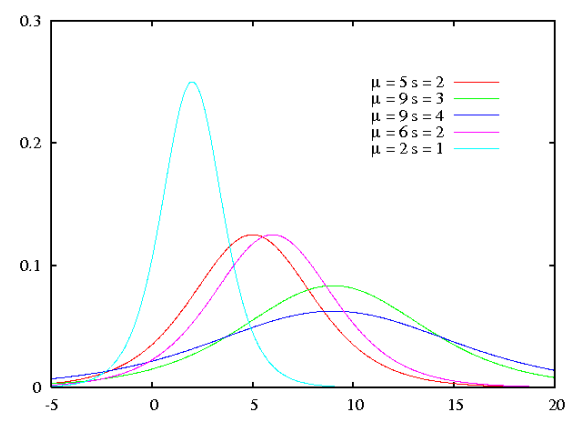
\includegraphics[scale=0.75]{images/logistic_distribution}
	\caption{Exemple de distribution logistique.}
\end{figure}

D'un point de vue mathématique, la densité de probabilité est donnée par :
$$f(x; \mu,s) = \frac{e^{-\frac{x-\mu}{s}}} {s\left(1+e^{-\frac{x-\mu}{s}}\right)^2}
=\frac{1}{s\left(e^{\frac{x-\mu}{2s}}+e^{-\frac{x-\mu}{2s}}\right)^2}$$
Les probabilités cumulées par :
$$F(x; \mu, s) = \frac{1}{1+e^{-\frac{x-\mu}{s}}} = \frac12 + \frac12 \;\operatorname{tanh}\!\left(\frac{x-\mu}{2s}\right)$$

Cette dernière a une forme semblable à une distribution Gaussienne, 
mais avec des queues épaisses et donc une \textit{kurtosis} plus élevée. La \textit{kurtosis} étant définie comme suit:
$$Kurt(X) = E\left[\left(\frac{X - \mu}{\sigma}\right)\right]$$
Où $\mu$ est la moyenne mathématique et $\sigma$ la déviation standard. 

Le but est de modéliser: $P(Y=1 | X=x)$ comme fonction de x. Nous voulons donc savoir quelle est la probabilité que 
la classe\footnote{Dans ce cas, la classe désigne une réalisation de la variable aléatoire $Y$.} $Y$ vaille $1$ sachant que $X$ vaut $x$.

Le modèle de régression est le suivant \cite{machine_learning_automated_trading}:
\begin{center}
$log(\frac{p(x)}{1 - p(x)}) = \beta_0 + x \cdot \beta$
\end{center}
, où $\beta_0$ représente l'ordonnée à l'origine de la régression linéaire
, $\beta$ est le coefficient de régression, de même dimension que $x$, et $x$ la donnée dont on veut obtenir la classe.

En résolvant cette équation pour $p$, cela donne \cite{machine_learning_automated_trading}:
\begin{center}
$p(x|y) = \frac{1}{1 + e^{-(\beta_0 + x \cdot \beta)}}$
\end{center}

\paragraph{}
Dans le cadre de l'article: \textit{A Machine Learning Approach to Automated Trading} \cite{machine_learning_automated_trading}, 
l'auteur a implémenté deux variations de cet algorithme:
\begin{itemize}
\item \textit{Logistic regression with a ridge penalty}:
\begin{center}
$$\sum_{i=1}^N (y_i - \sum_j\beta_j x_{ij})^2 + \lambda \sum_j \beta_j^2$$
\end{center}
, où $y_i$ est la classe de notre observation, $\beta_j$ sont les coefficients de la régression logistique originale \cite{machine_learning_automated_trading} et $x_{ij}$
sont les $j$ éléments de l'observation $i$.

L'objectif est de minimiser le carré de la différence entre la classe, ou résultat, de $y_i$ et le résultat 
calculé: $\sum\limits_j\beta_j x_{ij}$. Donc en fonction de l'observation $x_i$ et des coefficient de $\beta$.
En ajoutant une pénalité, sur $\beta$, on va tenter d'éviter le sur-apprentissage.

\item \textit{Lasso logistic regression/ Lasso regularization}:
\begin{center}
$$\sum_{i=1}^N (y_i - \sum_j\beta_j x_{ij})^2 + \lambda \sum_j |\beta|$$
\end{center}
Le fonctionnement est similaire au précédent, seul change la pénalité.

\end{itemize}

\paragraph{}
Comme mentionné plus haut, l'optimisation porte sur les paramètres de l'équation. Dans le cas de la régression logistique, 
il s'agît du $\beta$. Il conviendra donc de trouver la valeur optimale pour cette variable afin de maximiser ou minimiser 
les équations ci-dessus. De manière similaire pour les autres techniques de \textit{ML}, 
les équations et les paramètres vont changer, mais  le but sera toujours d'optimiser ces éléments. 

\subsubsection{Les arbres de décision}\label{section arbre de décision}

\paragraph{}
Un arbre de décision est un arbre, dont chaque nœud représente un test sur un attribut. 
Les branches qui suivent directement le nœud sont les valeurs possibles de l'attribut. 
Les feuilles de l'arbre, quant à elles, sont la classification d'élément donné en entrée.

Il est important de disposer des attributs avant de commencer la construction de l'arbre. 
Lors de l'implémentation, nous pouvons représenter l'arbre comme une suite de \textit{if-then-else} afin 
d'améliorer la lisibilité. Dans ce cas très précis, disposer d'un langage permettant le \textit{pattern matching} est fort utile.

Cet algorithme a tendance à très facilement sur-apprendre, il convient donc de bien choisir la manière de construire 
l'arbre ainsi que l'ensemble d'entraînement pour minimiser cet effet. 

Voici un exemple d'arbre de décision\footnote{\url{http://cloudmark.github.io/images/kotlin/ID3.png}}:
\begin{figure}[h!]
\centering
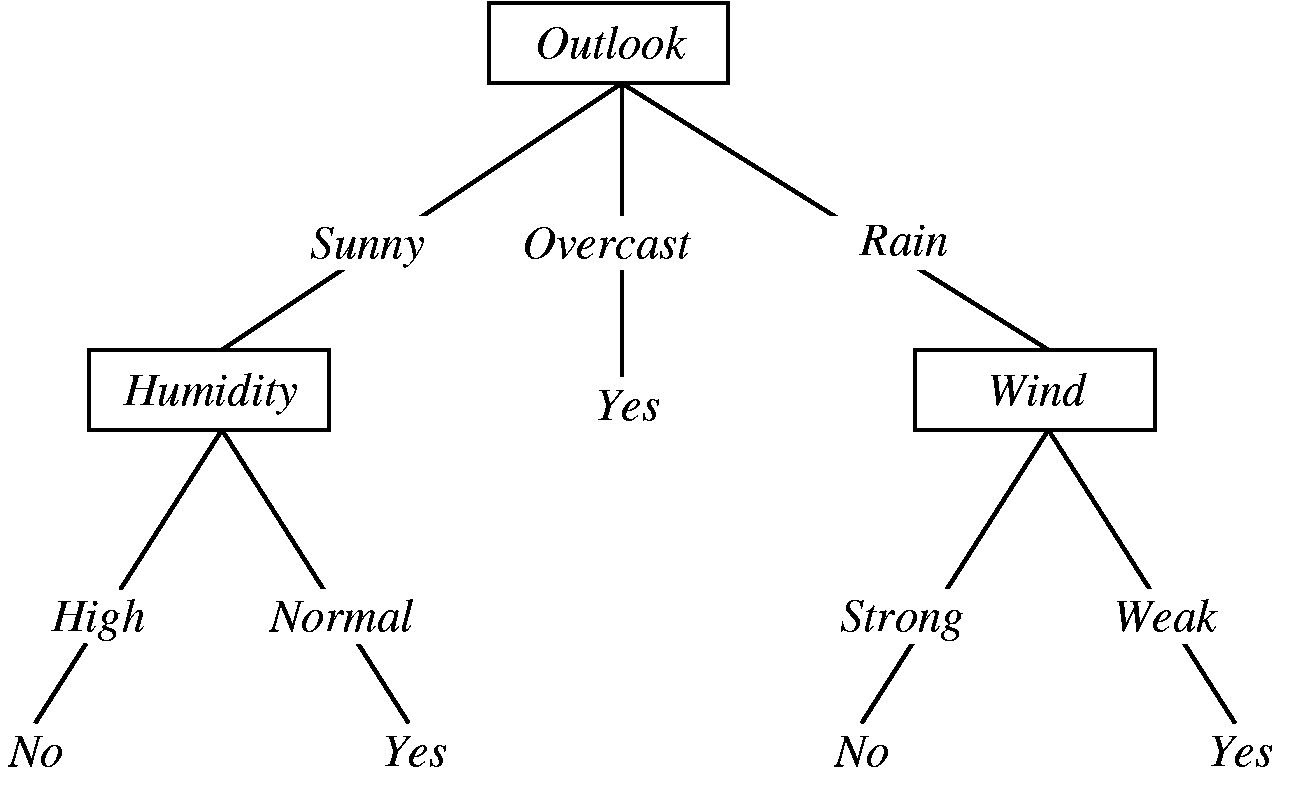
\includegraphics{images/exemple_tree}
\caption{Exemple d'arbre de décision: Permet de décider si nous pouvons aller jouer au tennis ou non.}
\end{figure}

\paragraph{}
Afin de construire l'arbre à partir de l'ensemble d'entraînement, il existe plusieurs algorithmes. 
Un des plus connus est le \textit{ID3} \cite{id3}. Il s'agit d'une méthode de type \textit{greedy}.

À chaque itération, il faut:
\begin{itemize}
 \item effectuer un test statistique\footnote{Il vise à vérifier la quantité d'information gagnée pour 
 la classification \cite{id3}.} afin de trouver l'attribut le plus discriminant.
 \item utiliser cet attribut comme nœud.
 \item retourner au premier point, tant que l'ensemble des attributs n'est pas vide.
\end{itemize}
Nous allons construire l'arbre de manière \textit{top-down} en utilisant ,à chaque pas, le meilleur attribut, selon notre test statistique. La construction de l'arbre constitue la phase d'entraînement. Si de nouvelles données viennent s'ajouter, il devient nécessaire de construire un nouvel arbre, soit une nouvelle phase d'entraînement.

La phase de classification consiste à parcourir l'arbre en appliquant les prédicats à l'instance que nous désirons classifier. Une fois arrivé a une feuille, nous avons un résultat.


\subsubsection{\textit{Naive Bayes}}\label{section naive bayes}
\paragraph{}
À l'instar de la régression logistique (voir \ref{section régression logistique}), il s'agit d'un classifieur probabiliste. 
Ce dernier se base sur le théorème de Bayes\footnote{\url{https://brilliant.org/wiki/bayes-theorem/}}:
\begin{center}
$P(Y|X) = \frac{P(X|Y)}{P(X)}P(Y)$
\end{center}

À partir de cela, nous obtenons l'équation de \textit{machine learning} suivante \cite{machine_learning_automated_trading}:
\begin{center}
$V_{NB} = arg\ max_{v_{j \in V}} P(v_j) \prod\limits_i P(a_i | v_j)$
\end{center}
Où $V_{NB}$ est la classe obtenue, $P(v_j)$ la probabilité à \textit{priori} donc sans informations 
et $\prod\limits_i P(a_i | v_j)$ la probabilité de vraisemblance.
Il convient donc de trouver la classe qui maximise ce calcul.

Afin d'avoir une certaine sécurité dans les résultats, il est possible d'ajouter un seuil. 
Les réponses du classifieur étant comprise entre $0$ et $1$, le seuil permettra de décider si la réponse sera prise en compte.

Par exemple, avec un seuil de $0.6$ si $V_{NB} = 0.58$, alors la réponse n'est pas validé et le classifieur ne renvoie aucun
résultat. Si $V_{NB} = 0.7$ alors la réponse est jugée sûre et la classe de $V_{NB}$ est retournée. 

\paragraph{}\label{section roc curve analysis}
La \textit{ROC\footnote{Receiver Operating Characteristic} Curve analysis} permet d'améliorer le classifieur. 
En effet cette dernière peut détecter les \textit{true positive rate} par rapport aux \textit{false positive rate} 
pour différents seuils de classification de l'algorithme \textit{Naive Bayes} \cite{machine_learning_automated_trading}. 
À partir de cela, nous pouvons déterminer le meilleur seuil de sortie et donc perfectionner notre algorithme.
De plus cette courbe peut aider à comparer des classifieurs entre eux en comparant 
la surface sous la courbe \cite{machine_learning_automated_trading}.

La méthode utilisée est la suivante \cite{machine_learning_automated_trading}: il faut faire s'intersecter 
la pente $S$ avec la courbe \textit{ROC} et ainsi obtenir une valeur optimale pour le seuil.
Cette pente $S$ est définie comme suit \cite{machine_learning_automated_trading}:
\begin{center}
$S = \frac{Cost(P|N) - Cost(N|N)}{Cost(N|P) - Cost(P|P)} \cdot \frac{N}{P}$
\end{center}
Sachant que $Cost(P|N)$ est le coût pour avoir mal classé une classe négative comme positive. 
$P$ est la somme des vrais positifs et des faux négatifs. $N$, quant à lui, 
vaut la somme des vrais négatifs ainsi que des faux positifs.

Voici une illustration\footnote{Source: \url{http://www.prolekare.cz/dbpic/jp_5403_f_20-x1000_1600}}:
\begin{figure}[H]
\centering
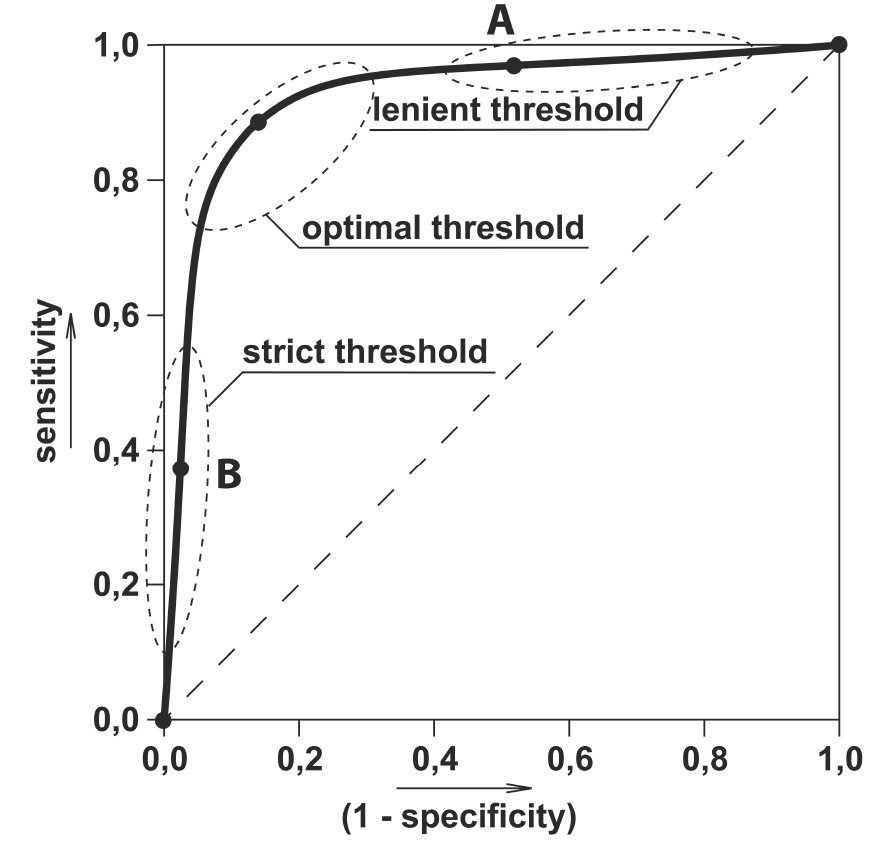
\includegraphics[scale=0.20]{images/roc_curve}
\caption{Exemple de \textit{ROC curve}: L'axe des $x$ correspond au taux de faux positifs et l'axe des $y$ 
au taux de vrais positifs. On veut donc tendre vers $y = 1$ et $x = 0$. Lors de l'optimisation par la pente $S$, 
le but sera d'obtenir une intersection avec la \textit{ROC curve} dans la zone \textit{optimal threshold} 
afin d'avoir le meilleur seuil possible.}
\end{figure}


\subsubsection{\textit{SVM}}\label{section svm}
\paragraph{}
Le but de l'algorithme \textit{SVM}\footnote{\textit{Support Vector Machine}} est de séparer les données grâce à un hyper-plan.
Cela permet de différencier les classes des observations suivantes en déterminant s'ils se trouvent d'un côté ou l'autre 
du plan. Ce dernier n'est pas unique\footnote{Source: \url{https://computersciencesource.files.wordpress.com/2010/01/svmafter.png}}: 
\begin{figure}[H]
\centering
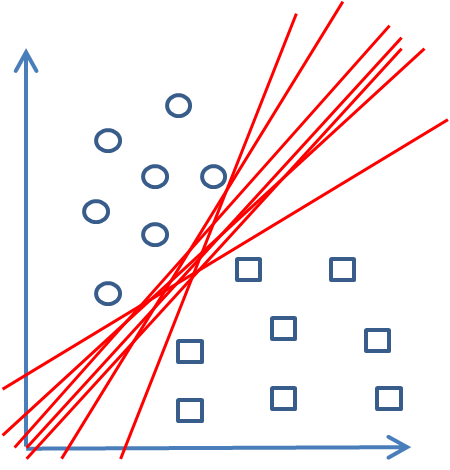
\includegraphics{images/svm_exemple}
\caption{Exemple d'hyper-plans séparant les données. Si nous voulons classifier un nouvel élément, 
il suffit de calculer s'il se trouve à gauche ou à droite de l'hyper-plan. Dans le premier cas, il s'agira, 
pour notre algorithme, d'un rond et dans l'autre d'un carré}
\end{figure}

\paragraph{}
Notre fonction est:
\begin{center}
$f(x) = (w \cdot x) + b$
\end{center}
Où $x$ est le vecteur\footnote{i.e notre instance.}, $w$ est le vecteur normal à l'hyperplan et $b$ l'ordonnée à l'origine.
Le but est de maximiser la distance entre les points les plus proches de l'hyper-plan, tout en pénalisant 
les points mal classés. Il n'est pas toujours possible de séparer les données de dimensions $n$, 
il conviendra donc d'augmenter la dimension afin d'obtenir une dimension $m > n$ plus discriminante. 
La fonction $\phi(x)$ est utilisée dans ce but. Un exemple de fonction est:
\begin{center}
$\phi: R^2 \rightarrow R^3 :(x, y) \rightarrow (x, y, z):= (x^2, \sqrt{2}x y, y^2)$
\end{center}

Il est possible d'imager cette opération comme cela\footnote{\url{https://www.dtreg.com/uploaded/pageimg/SvmDimensionMap.jpg}}:
\begin{figure}[H]
\centering
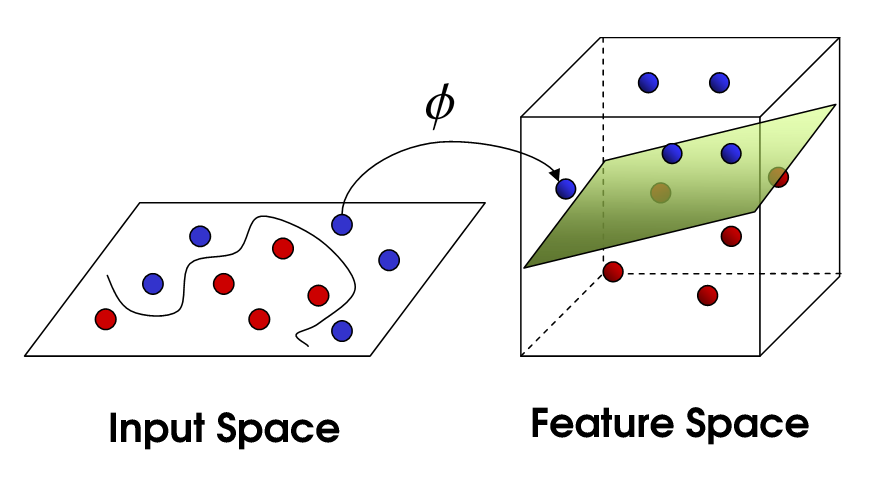
\includegraphics[scale=0.3]{images/svm_exemple_phi}
\caption{Exemple d'utilisation de la fonction $\phi$ pour passer d'un espace $R^2$ à $R^3$ afin de faciliter la séparation.}
\end{figure}


En terme d'équation, nous voulons minimiser w, dans l'équation de l'hyper-plan: $(w \cdot x) + b$. Il faut également prendre
en compte $y_i \in \{-1,+1\}$ :
\begin{center}
 \[ (w \cdot x) + b =
  \begin{cases}
    \ge +1   & \quad \text{si $y_i = +1$}\\
    \le -1 & \quad \text{si $y_i = -1$}\\
  \end{cases}
\]
\end{center}

 Ce qui donne \cite{svm_equation}:
\begin{center}
$y_i (w \cdot x_i + b) \ge 1$
\end{center}
Si malgré l'augmentation de la dimension, les données ne sont pas séparables, 
il faut tenter de minimiser le nombre d'éléments mal placés. Pour ce faire \cite{svm_equation}:
\begin{center}
$y_i (w \cdot x_i + b) \ge 1 - \xi_i$ avec $\xi_i > 0$ 
\end{center}
Afin de diminuer l'erreur et optimiser au mieux notre classifieur.


\subsubsection{Réseaux de neurones}
\paragraph{}
Tout comme les algorithmes génétiques s'inspirent de la sélection naturelle\cite{algorithme_genetique} dans un but d'optimisation,
les réseaux de neurones se basent sur un modèle formel de neurones
\footnote{Neurones formels: \url{http://www.peoi.org/Courses/Coursesfr/neural/neural3.html}} afin de copier la capacité 
d'apprentissage des êtres vivants.

Il s'agit d'opérer à partir de données en entrée, des \textit{inputs}, une ou plusieurs multiplications matricielles
en utilisant des vecteurs de poids, des \textit{weights}. L'optimisation s'applique sur les \textit{weights},
afin de maximiser la classification.

Un réseau de neurones peut avoir plusieurs couches, \textit{layers}. Dans ce cas, la première couche est
appelée \textit{input layer}, la dernière \textit{output layer} et toutes celles entre ces deux sont
les \textit{hidden layers}. De plus, les neurones peuvent être pleinement connectés avec ceux de la couche
suivante, \textit{feed-forward}; ce qui signifie que les neurones de la couche $n-1$ influencent ceux de
la couche $n$. Il est également possible que les éléments de $n$ agissent sur les neurones de $n-1$, ce
phénomène est appelé \textit{feedback networks}.

\begin{figure}[H]
\centering
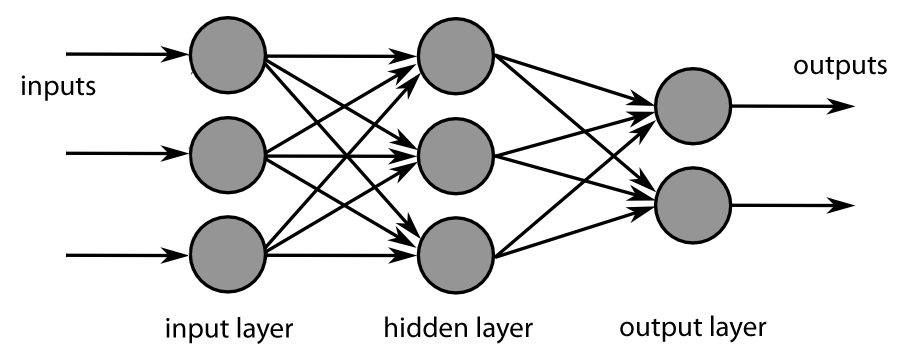
\includegraphics[scale=0.4]{images/neural_net_feedforward}
\caption[]{Exemple d'un réseau de neurones avec plusieurs couches. Illustre également
le \textit{feed-forward}: l'\textit{ouput} de l'\textit{input layer} est propagé dans chaque
neurones de l'\textit{hidden layer}. Même chose pour les deux dernières couches.\footnotemark}
\end{figure}

\begin{figure}[H]
\centering
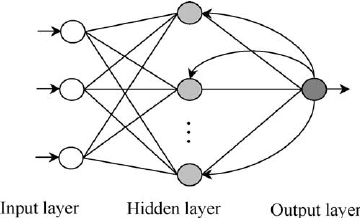
\includegraphics{images/neural_net_feedback}
\caption[]{Exemple d'un réseau de neurones avec plusieurs couches. Dans ce cas là,
les couches font du \textit{feed-forward} mais de plus, le \textit{feedback} est utilisé afin
d'influencer les couches précédant l'\textit{output layer}.\footnote[2]{}}
\end{figure}

\footnotetext{Source: \url{http://web.utk.edu/~wfeng1/spark/_images/fnn.png}}
\stepcounter{footnote}\footnotetext{Source:\url{https://jcrisch.files.wordpress.com/2015/04/reseau_de_neurones.png}}

\paragraph{}
Concernant la valeur de sortie, elle peut être simple, comme le résultat d'une classification binaire,\textit{i.e.} $0$ ou $1$
en sortie. Mais elle peut également être d'une dimensionnalité plus élevée comme un vecteur, citons l'exemple d'un point
dans un espace $R^2$.

Afin de borner les valeurs en sortie, la plupart des réseaux utilisent une fonction. Nous pouvons citer :
\begin{itemize}
\item La fonction sigmoïde : $S(t) = \frac{1}{1 + e^{-t}}$.
\item La fonction tangente hyperbolique : $f(x) = tanh(x)$.
\end{itemize}

Bien souvent, l'utilisation d'un réseau de neurones à une couche est suffisante. Cela est valable pour les fonctions continues,
dans le cas de fonctions discontinues, il est intéressant de passer à un réseau disposant de plusieurs couches.
Attention toutefois, si le nombre de neurones est trop important, l'algorithme va avoir tendance à sur-apprendre,
et à l'inverse, à sous-apprendre si le nombre est trop faible. Il est donc important de bien doser cette quantité afin
d'éviter ces problèmes.

\paragraph{}
Un exemple concret de réseau de neurones est celui présenté dans l'article qui se trouve au cœur du projet ~\cite{fx_trading}.
Avant de montrer les équations, en voici un schéma \cite{fx_trading}:
\begin{figure}[H]
 \centering
 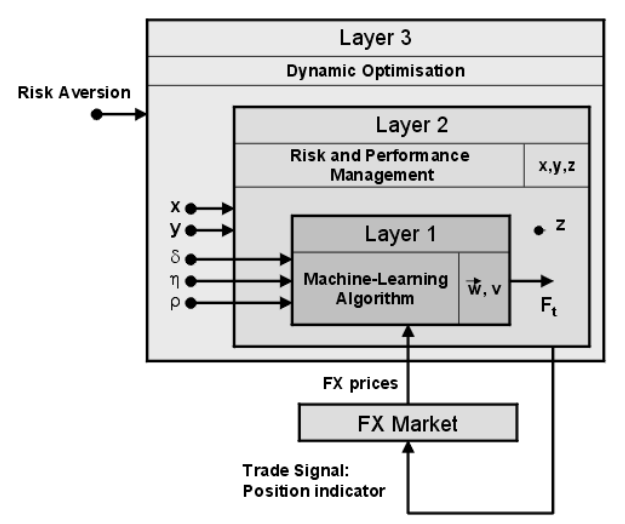
\includegraphics[scale=0.4]{images/exemple_nn_projet}
 \caption{Représentation sous forme de schéma du réseau de neurones. Avec $w$ le vecteur de poids, $v$ le seuil, $\delta$ le coût de
 \textit{trading}, $\eta$ un paramètre d'adaptation, $\rho$ le taux d'apprentissage, $x$ le seuil d'arrêt lors de pertes, $y$ le
 seuil de \textit{trading}, $z$ la condition d'arrêt automatique lors de pertes critiques et l'aversion au risque notée $\upsilon$.}
\end{figure}

Il s'agit de trois couches qui doivent optimiser chacune une série de paramètres. La première va maximiser le vecteur de poids $w$
ainsi que $v$ le seuil. À partir de ces paramètres, nous pouvons utiliser la formule suivante :
$$F_t = sign(\sum_{i=0}^M w_{i,t} r_{t-i} + w_{M+1,t} F_{t-1} + v_t)$$
où $r := p_t - p_{t-1}$ est le rendement d'une position. $F_t$ nous permet de calculer la position à prendre au temps $t$ en tenant
compte de l'historique des prix.

L'optimisation de $w$ se fait par un algorithme de descente du gradient (voir \ref{section descente du gradient}).

\paragraph{}
La deuxième couche va travailler à partir des paramètres $x,y,z$. Il est possible que le marché soit irrationnel durant une longue
durée, dans ce cas la psychologie peut pousser à garder une position en espérant un changement. C'est ce genre de comportement qu'un
algorithme permet d'éviter. Pour ce faire, nous définissons un excédant des pertes et nous veillons qu'il soit toujours à une distance
$x$ du meilleur prix atteint; afin d'éviter de tenir trop longtemps une position défavorable.

Il est également intéressant de définir un seuil. Si la réponse du réseau est supérieure à ce seuil, nous la prenons en compte et
dans le cas contraire, nous ne faisons rien. Cela permet d'évaluer la "force" du signal renvoyé par la première couche. Ce seuil
est $y$.

La dernière variable utilisée dans cette couche est $z$. Il y a un consensus dans la communauté de \textit{trading} concernant le fait
que les algorithmes fonctionnent bien durant un temps puis cesse d'être profitable. À ce moment, il convient d'arrêter le programme
et d'y apporter des modifications\footnote{Au niveau des équations, des données ou des paramètres.} avant de le relancer. La tâche du
paramètre $z$ est de donner un seuil pour les pertes du profit cumulé qui, lorsqu'il est dépassé, lance une procédure d'arrêt.
Contrairement à $x,y$ qui seront optimisés par la troisième couche, le paramètre $z$ est fixé au début du programme et ne change plus.

\paragraph{}
La couche d'optimisation dynamique est la troisième couche. Cette dernière va, à chaque itération, optimiser les paramètres suivants :
$x,y,\eta,\delta,\rho$.

Afin de conduire à bien l'optimisation, il fallu définir une fonction de coût\cite{fx_trading}:
$$\Sigma := \frac{\sum_{i=0}^N (R_i)^2 I(R_i < 0)}{\sum_{i=0}^N (R_i)^2 I(R_i > 0)}$$
$$ U(\overline{R},\Sigma,\upsilon) := a\cdot(1-\upsilon)\cdot \overline{R} - \upsilon \cdot \Sigma$$

,où $R_i := W_i - W{i-1}$ est le rendement au temps $i$ avec $W_i$ le profit cumulé, $\overline{R} := \frac{W_N}{N}$ est le profit moyen
avec $N$ qui est le nombre d'intervalle, $a$ une constante et $\upsilon$ l'aversion au risque.
Ces équations semblent complexes, néanmoins $\Sigma$ représente les \textit{returns} négatifs sur les positifs.

Ces équations ont été construites de manière à posséder ces propriétés \cite{fx_trading}:
\begin{itemize}
 \item Une stratégie négative implique un risque très élevé afin d'éviter de soudaines et importantes pertes.
 
 \item La mesure $\Sigma$ pénalise uniquement les stratégies négatives et pas les stratégies positives. 
\end{itemize}

La fonction à optimiser est donc :
$$\max_{\delta, \eta, \rho, x, y} U(\overline{R};\Sigma: \delta, \eta, \rho, x, y; \upsilon)$$

Car $x,y,\eta,\delta,\rho$ interviennent tous dans le calcul de $\Sigma$. Ces derniers peuvent être optimisés de la manière voulue.
\\
Les réseaux de neurones peuvent être optimisés de plusieurs manières. L'une d'entre elle est la descente du gradient.

\subsubsection{Descente du gradient}\label{section descente du gradient}
\paragraph{}
L'algorithme de descente du gradient fonctionne sur des fonctions réelles différentiables sur un espace tel
que $\mathbb{R}^n$. Il est itératif et fonctionne en améliorant l'itération précédente, jusqu'à
atteindre une condition d'arrêt.

Avant d'en expliquer la teneur mathématique, voici un exemple de l'algorithme dans $\mathbb{R}^2$ :

\begin{figure}[H]
\centering
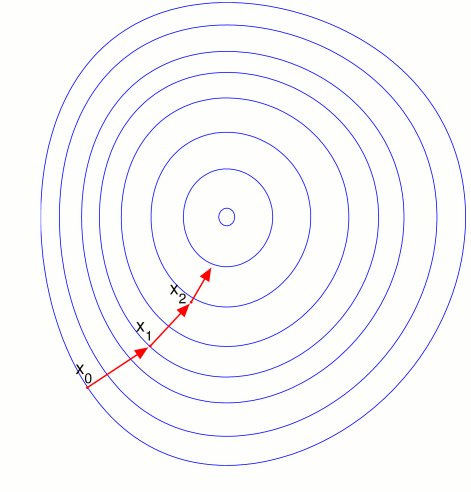
\includegraphics[scale=0.40]{images/descente_gradient_exemple}
\caption[]{Exemple de l'algorithme de descente du gradient en deux dimensions. À chaque itération,
il faut prendre la direction opposée au gradient\footnotemark, cela permet d'arriver à un nouveau
point. En itérant, on se rapproche de l'optimum. }
\end{figure}

\footnotetext{Dans cet exemple, il est possible de dire, qu'il faut prendre la normal de la courbe de niveau.}

\paragraph{}
Afin de comprendre, les divers algorithmes, il est important d'avoir les connaissances mathématiques
sur ce sujet. L'algorithme se définit comme suit\footnote{Inspiré de \cite{wikipedia_descente_du_gradient}.}:

\paragraph{}
Soit un point initial $x_0 \in \mathbb{R}$. Soit $\epsilon > 0$ un seuil de tolérance. L'algorithme définit
une suite d'itération $x_1,x_2,.. \in \mathbb{R}^n$, jusqu'à ce qu'un test d'arrêt soit satisfait.
Pour passer de $x_i$ à $x_{i+1}$, il faut :
\begin{itemize}
\item Calculer $\bigtriangledown f(x_k)$

\item Si $||\bigtriangledown f(x_k)|| \le \epsilon$ alors arrêt.

\item Sinon il faut calculer $\alpha_k$ par recherche linéaire\footnote{La recherche linéaire consiste à choisir une direction
 de descente afin de minimiser une fonction donnée jusqu'à atteindre l'optimum ou un seuil fixé 
\cite{wikipedia_recherche_lineaire}.} sur $f$ en $x_k$. Cette recherche se fait dans la direction opposée au gradient,
soit $-\bigtriangledown f(x_k)$. Une fois $\alpha_k$ calculé, il faut mettre à jour le
point itéré : $$x_{k+1} = x_k - \alpha_k \bigtriangledown f(x_k)$$
\end{itemize}

\paragraph{}
La preuve que la recherche dans la direction opposée au gradient induit une décroissance est la suivante.
Si la dérivée est non nulle\footnote{i.e: Si nous ne sommes pas déjà sur un maximum} au point $x$, $f'(x) \ne 0$. Soit
$$d = - \bigtriangledown f(x)$$
Puisque :
$$f'(x) \cdot d = \bigtriangledown f(x) \cdot -\bigtriangledown f(x) = - ||\bigtriangledown f(x) ||^2 < 0$$

L'égalité est strictement plus petite car la dérivée est non nulle par hypothèse. Cela implique que :
$$f(x -\alpha \bigtriangledown f(x)) < f(x)\text{,\ } \forall \alpha > 0$$

Nous avons donc que pour chaque itération, la valeur obtenue va décroître jusqu'à attendre un maximum, local ou global, ou le seuil $\epsilon$.

\paragraph{}
La descente du gradient d'un point de vue mathématique peut également être utilisée conjointement à un réseau de neurones. 
En effet dans cet article ~\cite{fx_trading}, les poids $w$ de la première couche, sont optimisés suivant cette formule :
$$w_{i,t} = w_{i-1,t} + \rho \bigtriangleup w_{i,t}$$

Où $t$ correspond au temps, $i-1$ à l'itération courante et $\rho$ le taux d'apprentissage.

De part la convergence de $w_i$ vers son optimum, cela permet, une fois cette valeur obtenue, de l'injecter
comme étant les poids d'un réseau de neurones.

\paragraph{}
Il existe deux types d'algorithme de descente du gradient :
\begin{itemize}
\item Le \textit{Batch Algorithm} a pour but de minimiser la fonction de coût qui aura été définie au préalable en utilisant 
toutes les données. Ce dernier peut prendre énormément de temps, de par son côté itératif, si l'ensemble d'entraînement croît.
\item Le \textit{Online Algorithm} va également minimiser une fonction de coût. Contrairement au \textit{Batch Algorithm}, il
prendra les exemples un à un. L'optimisation ne se fera que pour l'exemple courant puis recommencera sur une autre donnée. 
Cette manière de procéder s'applique aisément sur les gros volumes de données.
\end{itemize}

Provenant de cet article \cite{descente_du_gradient_stochastique}, voici des équations pouvant être minimisées dans
le cadre d'un programme de \textit{machine learning}.
Soit $(x_i,y_i)\text{,\ } i=1..N$, un ensemble de données. Notre fonction de coût est $l(y,y')$.
Cela représente le coût de prédire $y'$ quand la réponse est $y$. Moyennons cela sur tous les exemples :

$$E_N(f) = \frac{1}{N} \sum_{i=1}^{n}l(f_w(x_i),y_i)$$

Où $f_w$ est une fonction pondérée par un vecteur de poids $w$ que l'on cherche à optimiser.
Pour optimiser les poids, nous allons utiliser la descente du gradient :
$$w_{k+1} = w_k - \alpha_k \bigtriangledown f_{w_k}(x) \rightarrow w_{k+1} =
w_k -\alpha_k \sum_{i=1}^n \bigtriangledown Q ((x_i,y_i), w_k)$$

Où $Q(x,y) = l(f_w(x),y)$.

\paragraph{}
Comme mentionné plus haut, la technique de \textit{Batch Algorithm} devient lente lorsque le nombre de données augmente.
Pour pallier ce problème, il existe une technique : \textit{stochastic gradient descent}. C'est une méthode d'approximation
statistique de la descente du gradient.

Il convient de ne prendre qu'un seul couple au lieu de l'ensemble complet d'entraînement. La somme disparaît donc dans l'équation à minimiser :
$$w_{k+1} = w_k -\alpha_k \bigtriangledown Q ((x_i,y_i), w_k)$$
C'est donc une technique de \textit{Online Algorithm}. L'algorithme peut traiter des données à la volée car il n'a pas
besoin de se souvenir des exemples précédant.

Il est possible pour pénaliser la complexité de $w$ de rajouter un élément. Cela permet de borner quelque peu les valeurs des poids:
$$w_{k+1} = w_k -\alpha_k \bigtriangledown Q ((x_i,y_i), w_k) + \sigma P(w_k)$$

Où $\sigma > 0$ est un hyper-paramètre et $P$ peut valoir :
\begin{itemize}
\item \textbf{L1 norm} = $P(w) := \sum\limits_{i=1}^n |w_i|$
\item \textbf{L2 norm} = $P(w) := \frac{1}{2}\sum\limits_{i=1}^n w_i^2$
\item \textbf{Elastic Net} = $P(w) := \rho \frac{1}{2}\sum\limits_{i=1}^n w_i^2 + (1 - \rho) \sum\limits_{i=1}^n |w_i|$
\end{itemize}


\subsubsection{\textit{Majority vote}} \label{section majority vote}
\paragraph{}
Le \textit{majority vote} n'est pas strictement un algorithme de \textit{ML}. Il s'agît plutôt d'améliorer les résultats
en modifiant la manière d'utiliser certains des algorithmes pré-mentionnés.
Il est donc possible d'employer le \textit{majority vote} avec la régression logistique, les réseaux de neurones, etc.

\paragraph{}
Le principe est le suivant. Soit $E$ notre ensemble d'entraînement, soit $M = \{f_1, f_2, ...\}$ notre ensemble de
méthodes $f_i$ de \textit{machine learning}. Notons $M_E = \{f_{1_E}, f_{2_E}, ...\}$ notre ensemble de
méthodes $f_{i_E}$ entraînées.
 
\[ f_{i_E}(x) =
  \begin{cases}
    1       & \quad \text{si la classe calculée de $x$ est 1.}\\
    0  & \quad \text{si la classe calculée de $x$ est 0.}\\
    -1 & \quad \text{si aucune classe n'est trouvée ou si le seuil est insuffisant.}\\
  \end{cases}
\]

L'algorithme se comporte comme suit pour une observation $x$:
\paragraph{}
$\forall f_{i_E} \in M_E$, il faut calculer $f_{i_E}(x)$ et garder la classe résultante dans notre liste de résultat $R$.
Si $\exists\ classe_i \in R$, telle que $$\sum (classe_i \in R) > \frac{|M_E|}{2}$$

Alors cela signifie que la $classe_i$ est notre résultat, dans le cas contraire, l'algorithme ne donne aucune réponse.

\paragraph{}
L'algorithme va donc, à partir d'un ensemble de méthodes et d'une observation, calculer les classes. Si
une de ces dernières est représentée de manière majoritaire\footnote{\textit{i.e.} 50\% des voix + 1 voix}, le
programme retournera ce résultat. Si la majorité n'est pas atteinte, aucune classe n'est jugée valable et donc
aucune réponse ne sera rendue.

Cette technique réduit la composante individuelle des méthodes de \textit{ML} ainsi que le risque d'erreur. Si
une observation est mal classifiée, cela signifie que plus de la moitié des algorithmes ont fait une erreur.
Dans ce cas, il convient de changer les attributs utilisés ou l'ensemble d'entraînement car l'erreur ne
proviendra vraisemblablement pas d'un problème d'implémentation ou de la faiblesse de classification d'un algorithme particulier.

\subsubsection{\textit{Random Subset}} \label{section random subset}
\paragraph{}
À l'instar du \textit{majority vote}, le \textit{random subset} est une technique pour employer des méthodes de \textit{ML}.

\paragraph{}
Le principe est le suivant :

Il faut prendre $N$ différents ensembles de données\footnote{Il est possible de découper notre ensemble initial afin
d'atteindre ce critère.} du domaine concerné. Ils permettront d'entraîner un algorithme sur chacun d'entre
eux\footnote{Comme \textit{Naive Bayes} ou {SVM}.}. Nous disposerons donc de $N$ instances de l'algorithme de \textit{ML}
initial, mais avec un entraînement différent pour chacun, puis pour chaque observation, nous allons utiliser ces $N$ instances
afin d'obtenir un résultat de classification.

Comme pour le \textit{majority vote}, si une même classe est représentée une majorité de fois, le \textit{random subset} retournera ce résultat, et aucun le cas contraire.

\paragraph{}
Il est nécessaire d'avoir un grand jeu de données afin de fournir suffisamment d'échantillons aux instances pour qu'elles
apprennent correctement.
Une fois ce problème résolu, cette technique nous donne la possibilité d'utiliser au mieux l'ensemble d'entraînement.
En le fractionnant, cela permet d'entraîner les algorithmes avec des données différentes et donc d'augmenter
l'horizon de connaissance du programme.

De plus, le système de majorité promeut une qualité et une confiance accrue dans les résultats obtenus.


\subsection{\textit{Machine Learning} dans le cadre de la finance}\label{section machine learning finance}
\subsubsection{Introduction}
\paragraph{}
Avant de parler des performances des algorithmes mentionnés, il convient de préciser que ces derniers proviennent
de plusieurs articles différents. Ils ont donc été testés avec des paramètres ayant des valeurs disparates ainsi
que sur des données distinctes.
Il est donc très compliqué de comparer les résultats des algorithmes entre deux articles différents et
d'affirmer qu'une méthode est meilleure qu'une autre. 

Pour un même article, il sera possible de comparer les performances  cependant dans le cas contraire, ces
résultats serviront plutôt à illustrer la qualité intrinsèque des procédés. Avec un résultat de 80\%,
nous pourrons estimer que la performance est bonne, et l'inverse pour une valeur de 20\%.

\paragraph{}
Pour tous les algorithmes qui ont été mentionnés dans la section précédente, nous allons expliquer les changements
appliqués à ces derniers en vue de les étendre au domaine financier. De plus nous étudierons les résultats obtenus
et analyserons quelles améliorations apportent un gain significatif dans la classification.

La séparation sera quelque peu différente. Certains articles cumulant plusieurs algorithmes, afin d'éviter
les répétitions d'explications, il convient de les séparer par article afin de regrouper les améliorations.

De plus, tous les algorithmes ne sont pas forcément évalués dans les articles. Il est donc possible que certains
comme les réseaux de neurones n'aient pas de valeurs.

\subsubsection{\textit{A Machine Learning Approach to Automated Trading}}

\subsubsubsection{Introduction}
\paragraph{}
Cet article montre un exemple d'application sur le marché des actions \cite{machine_learning_automated_trading}
\footnote{Ou \textit{Stock market.}}. Après avoir essayé deux approches :
\begin{itemize}
\item L'approche individuelle.
\item L'approche par secteur.
\end{itemize}

La première partait de l'hypothèse que l'historique du prix d'une action contenait des motifs permettant la prédiction
du prix futur. Pour prédire $P_N$ l'auteur utilisait les $N$ précédant prix, soit : $[P_{N-1}, P_{N-2},...,P_1]$. Il s'agissait d'un modèle simple qui ne prenait pas en compte les actions des entreprises concurrentes.
Après les premiers résultats, l'auteur a conclu que cette approche
était trop simple pour être utilisée, car les valeurs étaient significativement moins bonnes que celle de la
seconde approche\cite{machine_learning_automated_trading}.

La seconde approche, quant à elle, repose sur la supposition que le prix d'une action dépend des autres actions,
souvent concurrentes. Il a donc pris en compte l'historique des prix du sous-jacent évalué, mais également celui de ses
concurrents en termes de marché. Les données possédées par l'auteur portent sur divers secteurs. Notamment celui
de l'\textit{utility}, de l'\textit{energy} et de l'\textit{information technology}. Le procédé est le suivant,
pour déterminer si une action précise $A_1$ va augmenter ou diminuer, il va analyser le prix de l'action durant les $N$ jours
précédant mais également celui des $M$ autres actions du secteur donné.
$$f(A_{(1,t_1)},\dots, A_{(1,t_N)}, A_{(2,t_1)}, \dots, A_{(2,t_N)}, \dots, A_{(M,t_1)},\dots,A_{(M,t_N)}) = A_{(1,t_0)}$$

\paragraph{}
Un autre point qu'il convient d'aborder porte sur l'ensemble d'entraînement. Afin d'entraîner et d'évaluer son programme,
il a fallu partager le \textit{set} de données.

Dans le cas contraire, il aurait été impossible de tester les algorithmes entraînés. Ou bien, ils auraient été évalués
sur les mêmes données que leur entraînement. Ce qui n'est pas possible.

Le choix a donc été fait de partager l'ensemble de données en deux sous-parties. Une première contenant 80\% des
données qui sera dédiée à l'entraînement et une seconde avec 20\% pour l'évaluation.

\paragraph{}
L'auteur a utilisé le S\&P\footnote{Le \textit{Standard \& Poor's} est un indice calculé à partir de 500 grandes
sociétés capitalisées dans les bourses américaines.} pour sélectionner des actions. Les données du secteur \textit{utility} en
contiennent 29, le secteur {energy} 39 et le secteur \textit{technology} 61. Tous les \textit{ticks} entre
le 02.01.2014 et le 01.02.2016 sont présents dans les données. La taille de l'historique est de quatre jours afin
que les vecteurs d'attributs ne soient pas trop grand.

Le but est donc à partir des quatre premiers jours de la semaine, de prédire si l'action sera en hausse ou non le cinquième jour.
\paragraph{}
Les trois métriques utilisées sont :
\begin{itemize}
\item Le \textit{True Positive Rate} est définit comme suit :
$$\textit{TPR} = \frac{\textit{TP}}{\textit{TP} + \textit{FN}}$$
Où \textit{TP} sont les positif détectés positifs et \textit{FN} les négatifs détectés positif.
\item Le \textit{True Negative Rate} est définit comme :
$$\textit{TNR} = \frac{\textit{TN}}{\textit{TN} + \textit{FP}}$$

\item Le \textit{True Rate} :
$$\textit{TR} = \frac{\textit{TP} + \textit{TN}}{\textit{TP} + \textit{TN} + \textit{FP} + \textit{FN}}$$
\end{itemize}

\subsubsubsection{Résultats}
Cet article a pour avantage de tester de nombreux algorithmes et techniques. En analysant les résultats, des pistes peuvent être mises en évidences. Nous pourrons également déterminer un ordre de grandeur concernant la précision pour un problème donné.
\paragraph{}
Les résultats proviennent de l'article suivant \cite{machine_learning_automated_trading} :

\begin{table}[h!]
	\centering
\begin{tabular}{|l|l|l|l|}
	\hline
	\ & \textit{TPR} & \textit{TNR} & \textit{TR}\\
	\hline
	\textit{Utility} & 0.5595 & 0.4507 & 0.5235 \\
	\hline
	\textit{Energy} & 0.4653 & 0.5369 & 0.5047\\
	\hline
	\textit{Information Technology} & 0.5244 & 0.5031 & 0.5102\\
	\hline
\end{tabular}
\caption[]{Tableau de résultats pour l'algorithme \textit{Lasso Logistic Regression} (voir \ref{section régression logistique}).}
\end{table}



\begin{table}[h!]
	\centering
\begin{tabular}{|l|l|l|l|}
	\hline
	\ & \textit{TPR} & \textit{TNR} & \textit{TR}\\
	\hline
	\textit{Utility} & 0.5699 & 0.4624 & 0.5179 \\
	\hline
	\textit{Energy} & 0.4524 & 0.5320 & 0.5042\\
	\hline
	\textit{Information Technology} & 0.5075 & 0.54966 & 0.5052\\
	\hline
\end{tabular}
\caption[]{Tableau de résultats pour l'algorithme \textit{Decision Tree} (voir \ref{section arbre de décision}).}
\end{table}



\begin{table}[h!]
	\centering
\begin{tabular}{|l|l|l|l|}
	\hline
	\ & \textit{TPR} & \textit{TNR} & \textit{TR}\\
	\hline
	\textit{Utility} & 0.5949 & 0.4957 & 0.5495 \\
	\hline
	\textit{Energy} & 0.4797 & 0.5812 & 0.5193\\
	\hline
	\textit{Information Technology} & 0.5115 & 0.5048 & 0.5091\\
	\hline
\end{tabular}
\caption[]{Tableau de résultats pour l'algorithme \textit{Naive Bayes} (voir \ref{section naive bayes}).}
\end{table}


\begin{table}[H]
	\centering
\begin{tabular}{|l|l|l|l|}
	\hline
	\ & \textit{TPR} & \textit{TNR} & \textit{TR}\\
	\hline
	\textit{Utility} & 0.5804 & 0.5081 & 0.5562 \\
	\hline
	\textit{Energy} & 0.4818 & 0.6049 & 0.5201\\
	\hline
	\textit{Information Technology} & 0.5142 & 0.5040 & 0.5149\\
	\hline
\end{tabular}
\caption{Tableau de résultats pour l'algorithme \textit{SVM} (voir \ref{section svm}).}
\end{table}


\paragraph{}
À ce stade, nous remarquons que les performances de la régression logistique et des arbres de décisions sont du même
ordre de grandeur. Ces derniers étant battus par les algorithmes \textit{Naive Bayes} et \textit{SVM}.

Un autre point important concernant le fait que les algorithmes détectent mieux les \textit{TPR} que les
\textit{TNR}\footnote{Exception faite du secteur énergie.}. Cela est dû au cours des actions des différents secteur
globalement en hausse dans les données prises en compte. Du coup, de par le manque de données à la baisse dans
l'ensemble d'entraînement, l'apprentissage est limité. Concernant le secteur de l'énergie, vu qu'il était en baisse,
l'inverse se produit.

Afin d'améliorer cet aspect l'auteur a utilisé le \textit{majority vote} avec les quatre algorithmes
\footnote{Source des résultats: \cite{machine_learning_automated_trading}}:

\begin{table}[h!]
	\centering
\begin{tabular}{|l|l|l|l|}
	\hline
	\ & \textit{TPR} & \textit{TNR} & \textit{TR}\\
	\hline
	\textit{Utility} & 0.5807 & 0.4921 & 0.5573 \\
	\hline
	\textit{Energy} & 0.4753 & 0.6003 & 0.5192\\
	\hline
	\textit{Information Technology} & 0.5133 & 0.5055 & 0.5233\\
	\hline
\end{tabular}
\caption{Tableau de résultats pour le \textit{majority vote} (voir \ref{section majority vote}).}
\end{table}

Les résultats sont similaires à ceux de \textit{Naive Bayes} et de \textit{SVM}, cela n'est donc pas très
concluant comme amélioration. Il est possible que les deux algorithmes ayant les meilleurs résultats sont
souvent d'accord sur la classe, cassant ainsi l'intérêt du vote.

\paragraph{}
L'auteur va utiliser l'algorithme \textit{Naive Bayes} afin de l'améliorer. En se concentrant sur un seul algorithme,
il lui est plus facile d'en voir les effets\footnote{Source des résultats: \cite{machine_learning_automated_trading}}.

\paragraph{}
\begin{table}[h!]
	\centering
\begin{tabular}{|l|l|l|l|}
	\hline
	\ & \textit{TPR} & \textit{TNR} & \textit{TR}\\
	\hline
	\textit{Utility} & 0.5949 & 0.4957 & 0.5495 \\
	\hline
	\textit{Energy} & 0.4797 & 0.5812 & 0.5193\\
	\hline
	\textit{Information Technology} & 0.5115 & 0.5048 & 0.5091\\
	\hline
\end{tabular}
\caption{Tableau de résultats pour l'algorithme \textit{Naive Bayes} (voir \ref{section naive bayes}) avec une optimisation
par \textit{ROC curve analysis} (voir \ref{section roc curve analysis}).}
\end{table}

Le fait d'utiliser la \textit{ROC curve analysis} afin d'obtenir le seuil optimal permet principalement d'augmenter
la performance dans la détection des négatifs. Il est important de mentionner que cela n'influence que peu
la détection des positifs car ils sont bien représentés dans l'ensemble d'entraînement et donc mieux reconnus.
L'amélioration est donc intéressante car sans augmenter le risque de sur-apprentissage, elle augmente la qualité
de classification.

\begin{table}[h!]
	\centering
\begin{tabular}{|l|l|l|l|}
	\hline
	\ & \textit{TPR} & \textit{TNR} & \textit{TR}\\
	\hline
	\textit{Utility} & 0.6021 & 0.5187 & 0.5779 \\
	\hline
	\textit{Energy} & 0.4574 & 0.5871 & 0.5108\\
	\hline
	\textit{Information Technology} & 0.5348 & 0.5317 & 0.5382\\
	\hline
\end{tabular}
\caption{Tableau de résultats pour le \textit{Random Subset} (voir \ref{section random subset}) avec l'algorithme 
\textit{Naive Bayes} (voir \ref{section naive bayes}) optimisé par \textit{ROC curve analysis} 
(voir \ref{section roc curve analysis}).}
\end{table}

L'amélioration est assez importante par rapport à l'algorithme \textit{Naive Bayes Roc curve analysis}. 
Le \textit{Random Subset} obtient 58\% et 54\% pour l'\textit{utility} et l'{information technology}, pour seulement 
55\% et 51\% au \textit{Naive Bayes ROC curve analysis}. Même s'il y a une légère perte pour le secteur 
\textit{energy} d'environ 1\%.
L'ensemble procure de meilleurs résultats.

\subsubsection{\textit{Online Machine Learning Algorithms For Currency Exchange Prediction}}

\subsubsubsection{Introduction}
\paragraph{}
Un autre exemple d'article utilisant les techniques de \textit{machine learning}. Ce dernier ayant principalement exploré la technique de la descente du gradient 
(voir \ref{section descente du gradient}) et plus précisément de sa version probabiliste ou
\textit{stochastic gradient descent} \cite{descente_du_gradient_stochastique}.

Trois variations ont été implémentées et testées :
\begin{itemize}
\item La descente du gradient stochastique simple ou \textit{Plain Stochastic Gradient Descent}\footnote{Noté: \textit{plainSGD}.}.
\item La descente du gradient stochastique avec choix aléatoire ou \textit{Stochastic Gradient Descent with random sample picking}\footnote{Noté: \textit{approxSGD}.}.
\item La descente du gradient stochastique avec choix aléatoire et "départ chaud" ou \textit{Stochastic Gradient Descent with random sample picking and warm start}\footnote{Noté: \textit{approxWarmSGD}.}.
\end{itemize}

\paragraph{}
Le \textit{random sample picking} est une technique qui consiste à choisir aléatoirement un élément d'un ensemble
de manière non uniforme. Dans ce cadre précis, il est intéressant d'accorder plus de valeurs à une donnée
récente qu'à une plus ancienne. On considère que les éléments proches de nous d'un point de vue temporel,
ont une plus grande influence.

La meilleure manière d'appliquer cela est d'utiliser une sélection aléatoire exponentielle.

\begin{figure}[H]
\centering
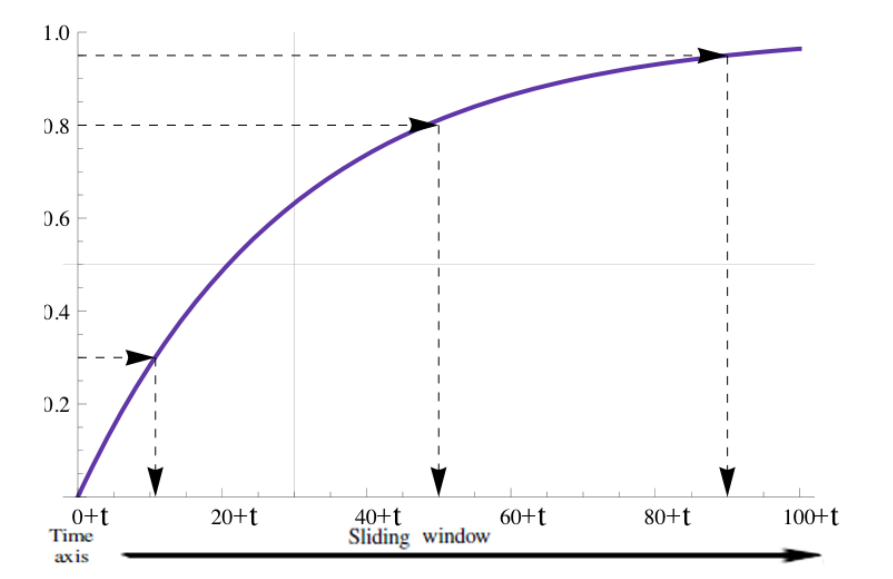
\includegraphics[scale=0.40]{images/choix_exp}
\caption[]{Exemple de distribution exponentielle\footnotemark.
Cela va donc permettre de choisir les points les plus proches avec une probabilité plus grande.}
\end{figure}

\footnotetext{Source: \cite{descente_du_gradient_stochastique}}

\paragraph{}
L'autre point important est le \textit{warm start}. C'est une pré-optimisation.
Il s'agît d'initialiser les paramètres du gradient d'une certaine manière afin d'augmenter la vitesse et les chances
de convergence. Pour ce faire, la meilleure option trouvée dans l'article consiste à utiliser les valeurs obtenues lors de la précédente itération
\cite{descente_du_gradient_stochastique}.
Par conséquent, l'algorithme convergera plus vite pour un coût plus faible en termes d'erreur de calcul.

\paragraph{}
La métrique d'évaluation est différente des notions de \textit{TPR},\textit{TNR} et \textit{TR}.
Dans cet article, le but est de prédire le prix d'un cours, comme EUR/USD à partir de plusieurs autres,
comme EUR/CAD, EUR/AUD, EUR/GBP. Il est donc extrêmement compliqué de calculer avec plusieurs décimales
le résultat exact, impliquant donc des taux nuls pour chacune des métriques.
Il fallu donc trouver une méthode basée sur l'erreur relative :
$$relative_{error} = \frac{\Delta x}{x}$$

Cela quantifie la différence entre le résultat calculé et le résultat réel tout en le pondérant.

\subsubsubsection{Résultats}
\paragraph{}
Tout comme l'article précédent, l'analyse des résultats et des algorithmes utilisés peuvent conduire à des pistes de recherches.
Le but est de calculer un taux de change à partir de données. Pour obtenir ces résultats précis, l'auteur a pris le
\textit{Singapore Hedge Fund FOREX Data Set} ainsi que le \textit{Capital K FOREX Data Set}. Les dates ainsi que la fréquence
ne sont pas précisées dans l'article.

L'algorithme retourne deux valeurs : le \textit{bid} et le \textit{ask} à partir des données fournies. Ci-dessous, nous allons
voir la précision de ces résultats. Les tableaux représentent la
comparaison entre les valeurs calculées et les valeurs réelles, soit l'erreur relative.

\begin{table}[H]
	\centering
\begin{tabular}{|l|l|l|l|}
	\hline
	Données & \textit{plainSGD} & \textit{approxSGD} & \textit{approxWarmSGD}\\
	\hline
	\ & \textit{Bid/Ask} & \textit{Bid/Ask} & \textit{Bid/Ask} \\
	\hline
	\textit{Singapoore with SW-1\footnotemark{}} & 0.1366274551\% & 0.133887583\% & 0.2294997927\% \\
	\hline
	\textit{Singapoore with SW/2\footnotemark{}} & 0.1366274551\% & 0.09281447603\% & 0.1551851906\%\\
	\hline

\end{tabular}
\caption[]{Tableau de résultats\footnote[3]{} pour les différentes versions de \textit{SGD} sur le
\textit{FOREX} de Singapore. Les différences entre le \textit{bid} et le \textit{ask} étant minimes,
l'auteur ne les a pas consignées.}
\end{table}

 \addtocounter{footnote}{-2} %3=n
\stepcounter{footnote}\footnotetext{$SW-1$ signifie une fenêtre de choix de taille $N-1$.}
\stepcounter{footnote}\footnotetext{$SW/2$ signifie une fenêtre de choix de taille $N/2$.}
\stepcounter{footnote}\footnotetext{Source des résultats: \cite{descente_du_gradient_stochastique}.}



\paragraph{}
Les erreurs relatives sont très faibles. Les estimations sont donc très proches des valeurs réelles. De plus, on
remarque que le  changement de la taille de la \textit{SW} peut avoir une grande influence. Sur le \textit{plainSGD}
cela ne change rien, on peut donc en conclure que les $N/2 - 1$ données supplémentaires ne sont pas significatives
dans le calcul. Pour le \textit{approxSGD} et le \textit{approxWarmSGD}, le taux d'erreur diminue. Nous pouvons donc
dire que la fenêtre était trop grande et, pire encore, ajoutait du bruit rendant le calcul moins précis.

D'un point de vue calculatoire c'est très intéressant car il est possible de diminuer la taille de la fenêtre et
donc gagner en vitesse tout en gardant, voir en augmentant, la qualité des résultats.


\begin{table}[H]
	\centering
\begin{tabular}{|l|l|l|l|}
	\hline
	Données & \textit{plainSGD} & \textit{approxSGD} & \textit{approxWarmSGD}\\
	\hline
	\ & \textit{Bid/Ask} & \textit{Bid/Ask} & \textit{Bid/Ask} \\
	\hline
	\textit{Capital K SW-1} & 0.01167\%/0.0117\% & 0.0116\%/0.0117\% & 1.502e-03\%/1.554e-03\% \\
	\hline
	\textit{Capital K SW/2} & 0.01167\%/0.0117\% & 0.0314\%/0.0313\% & 1.701e-03\%/1.751e-03\%\\
	\hline

\end{tabular}
\caption[]{Tableau de résultats\footnote{} pour les différentes versions de \textit{SGD}.}
\end{table}

\footnotetext{Source des résultats: \cite{descente_du_gradient_stochastique}}

\paragraph{}
Nous constatons qu'il n'y a pas de différence pour le \textit{plainSGD} entre les deux tailles de fenêtres. On
remarque cependant que pour les deux autres variantes, la diminution de la taille les pénalise. Cependant, l'ordre
de grandeur des erreurs demeure faible. Il est donc important de savoir si nous voulons un chiffre précis ou obtenir
le résultat de manière rapide. L'objectif aiguillera le choix pour l'une ou l'autre des fenêtres.

À noter, que le \textit{approxWarmSGD} obtient de meilleures valeurs que ces concurrents et subit beaucoup moins
les effets de la diminution de \textit{SW} que le \textit{approxSGD}.

\subsection{Conclusion}
\paragraph{}
Afin d'élaborer des algorithmes de \textit{ML}, il est important de saisir les considérations théoriques.
À partir de ces connaissances, le choix d'un algorithme est plus aisé. En effet, si vous voulez apprendre une fonction
continue, mieux vaut utiliser des techniques de descente de gradient et dans le cas de données faiblement différentiables, 
l'utilisation d'un programme \textit{SVM} avec un \textit{kernel trick} est recommandée.

Cela est également valable pour sa mise en place. Les optimisations mathématiques possibles sont nombreuses et complexes,
comme nous l'avons vu dans la partie (\ref{section machine learning finance}), il conviendra donc de les comprendre afin de
mieux cerner les contraintes et les gains lors de l'optimisation.

Ces éléments peuvent être vus comme une boîte à outils algorithmiques, le choix et l'utilisation des différents
outils reviendra à la personne qui programmera. Ce sera cette dernière qui devra construire l'algorithme le plus
adapté avec les données, les contraintes et les techniques à sa disposition.

\paragraph{}
Les considérations mathématiques ne sont pas les seuls éléments importants. Appliquer un algorithme sans chercher à comprendre
les cas concrets peut mener à des programmes peu efficaces.

Dans chacun des articles, les auteurs avaient une connaissance et une compréhension du monde de la finance suffisante,
pour améliorer les techniques en dehors du carde mathématique. L'approche par secteur \cite{machine_learning_automated_trading}
ou l'utilisation de méta-paramètres propre au domaine financier ~\cite{fx_trading} en sont des exemples concrets.
Chacun de ces éléments a sensiblement amélioré les performances des algorithmes auxquels ils ont été appliqués.

Une technique de \textit{machine learning} n'est qu'une solution à un problème mathématique précis. L'ajout d'éléments,
comme ceux cités auparavant, améliore la quantité d'informations disponible et précise l'équation mathématique à optimiser.

\paragraph{}
Il est important de lier ces deux parties pour obtenir des résultats optimaux.

Les valeurs peuvent être encourageantes même s'il convient de relativiser les résultats. Ces derniers ayant pu
être obtenus sur des ensembles de données "faciles". Ce mot qualifie des périodes avec peu de changements ou peu de
variations, ce qui facilite grandement la classification.
Néanmoins, les taux d'erreurs sont faibles et la classification efficace.
Cela démontre que les bons algorithmes appliqués avec une bonne connaissance du domaine fournissent des résultats satisfaisants. 

\paragraph{}
Le choix d'implémenter l'algorithme de réseau de neurones provient des justifications suivantes :
\begin{itemize}
 \item Les \textit{Neural Nets} peuvent, avec assez de ressources\footnote{Cela comprend le temps et les données.}, approximer n'importe
 quel fonction. De plus ils sont capables d'opérer des séparations non linéaires sans recourir au \textit{Kernel trick}.
 \item Il est possible d'éviter les problèmes de sur-apprentissage, en modifiant les méta-paramètres. Cela nous permet de profiter
 de n'importe quel ensemble d'entraînement sans craindre que ce dernier pose problème.
\end{itemize}

Les algorithmes d'arbres de décision sont des classifieurs linéaires. Ce qui signifie qu'ils sont limités
lorsque les données ne sont pas linéaires, réduisant de fait, la qualité de classification. On retrouve ce même problème
pour la régression logistique. De plus les arbres de décision (voir \ref{section arbre de décision}) ont de gros risques
de sur-apprentissage même avec un ensemble d'entraînement adapté, sans compter qu'ils gèrent mal les exemples en continus.
En effet, lors d'un entraînement \textit{online}\footnote{Quand les exemples arrivent de manière continue.} chacun des nouveaux
éléments peut introduire des exceptions. Ce qui implique de reconstruire l'arbre, ce cas pouvant être très lourd en termes
de calculs, il convient donc de l'éviter.

Le classifieur \textit{Naive Bayes} aurait pu être une méthode de classification efficace\footnote{i.e: Deviner si le cours va monter, descendre ou stagner.}car ce dernier peut classifier les données non linéaires,
ne présente pas de problème de sur-apprentissage et est adapté pour un apprentissage \textit{online}. Il suffit de rajouter le
dernier exemple dans l'équation pour mettre à jour l'apprentissage. La raison qui nous a poussé à choisir les réseaux de neurones 
plutôt que l'algorithme de \textit{Naive Bayes} est que ce dernier a des performances limitées sur un grand ensemble de données.
Si l'on prend des petits jeux de données, \textit{Naive Bayes} est très efficace
\footnote{Dans ce cadre précis, il est même meilleur que tous les autres algorithmes vus dans ce projet.}
\cite{ml_petites_donnees}.
Cependant si l'ensemble grandit, ces performances plafonnent, ce qui n'est pas le cas du \textit{Neural Nets} dont les
résultats augmentent à mesure que le nombre de données disponibles croît.

Au vu des raisons susmentionnées, un algorithme de réseau de neurones nous semblait un choix raisonnable tant pour les spécifications mathématiques que pour la manière de l'utiliser. Car le \textit{FOREX} nous
fournit suffisamment de données pour avoir d'excellent résultats, de plus, nous ne sommes pas limités par une classification linéaire.
Le cas échéant, si les réseaux de neurones ne fournissent pas de résultats suffisants, il sera possible de réorienter notre choix sur une autre méthode. Cela nous laisse des pistes de recherches tant en cas de succès que d'échec.


\newpage
%%%%%%%%%%%%%%%%%%%%%%%%%%%%%%%%%%%%%%%%%%%%%%%%%%%%%%%%%%%%%%%%%%%%%%%%%%
% début du projet  %%%%%%%%%%%%%%%%%%%%%%%%%%%%%%%%%%%%%%%%%%%%%%%%%%%%%%%
%%%%%%%%%%%%%%%%%%%%%%%%%%%%%%%%%%%%%%%%%%%%%%%%%%%%%%%%%%%%%%%%%%%%%%%%%%
\section{Projet}
\subsection{Introduction}
\paragraph{}
Le but de ce projet est d'implémenter l'algorithme présenté dans l'article \textit{"An automated fx trading system using adaptive
reinforcement learning"} \cite{fx_trading}. Notre question de recherche consiste à déterminer et à mesurer si les propositions informatiques
fonctionnent ou non et, le cas
échéant, de comprendre les raisons de ces résultats puis proposer des améliorations pour le faire fonctionner ou augmenter ces performances.

L'algorithme n'est pas totalement décrit car l'article
est un \textit{proof of concept} et n'a pas vocation à être publié comme une nouvelle méthode de \textit{trading}. Il s'agît plutôt d'une piste 
éventuelle de recherches. Il faudra donc
interpréter les éléments et interpoler ceux manquants. Une fois le programme créé, nous le testerons sur des données réelles afin d'estimer s'il est
utilisable ou non d'après des critères de \textit{back-testing}. Toutes les notions économiques, mathématiques et scientifiques nécessaires à la 
compréhension sont décrites dans l'état de l'art précédant cette partie. Néanmoins, les équations importantes seront introduites ou exposées à nouveaux
dans un soucis de rigueur scientifique et pour mieux comprendre les implications.

Cet algorithme est composé de trois parties. La première qui constitue le cœur du \textit{machine learning} présent, se base sur un réseau de neurones
à une couche construite de manière à utiliser la \textit{back-propagation} et le \textit{feed-forward}. L'optimisation des poids se fait via une descente du gradient simple 
à partir de fonctions de coût utilisant au mieux les données économiques à dispositions. La deuxième couche utilise des notions financiers afin de
déterminer si le signal obtenu par la couche une doit être utilisé ou non et comment limiter les risques et pertes. La dernière partie va permettre de
réduire l'influence humaine en optimisant les métas-paramètres. Ces derniers sont des paramètres qui conditionnent le comportement du réseau de neurones,
de la descente du gradient et de la deuxième couche. Comme le taux d'apprentissage $\rho$, le \textit{stop loss} $x$, etc.\footnote{Tous les métas-paramètres
seront introduits et expliqués dans la section suivante.} Ils ne varient pas 
à l'intérieur des dîtes parties et sont modifiés dans la troisième couche. Cela permet au programme d'avoir plus de flexibilité et d'adaptabilité par
rapport au temps et aux nouveaux éléments rencontrés.

À cause du caractère empirique du projet, nous avons dû chercher et expérimenter afin de comprendre, d'implémenter, d'interpoler et de corriger
les bouts d'algorithmes présentés dans le \textit{proof of concept} \cite{fx_trading}. Nous allons donc découper l'article de manière à pouvoir 
expliquer l'idée mais également les problèmes et nos améliorations.
Dans un premier temps, nous exposerons chacune des trois couches avec une partie présentant le concept mathématique et une autre pour la manière dont nous
l'avons implémentée. Ensuite, nous parlerons des problèmes rencontrés ainsi que les remédiations ou les pistes de solutions que nous avons trouvées.
Puis, nous présenterons les résultats, ainsi que certaines métriques afin d'expliquer les performances et le comportement de l'algorithme. Pour
finir, nous conclurons notre rapport en synthétisant les idées, les problèmes et les résultats et en proposant des améliorations ou des pistes pour 
des recherches futures.

\subsection{Algorithme}
Dans cette section, pour chacune des parties de l'algorithme, nous allons dans un premier temps expliquer son fonctionnement théorique et ses bases
mathématiques, puis exposer la manière dont nous avons implémenter ces éléments.
Une fois l'algorithme détaillé, nous présenterons les problèmes rencontrés ainsi que les remédiations proposées. Après nous passerons à l'analyse des
résultats pour les différentes variantes afin de saisir les causes et les conséquences de nos choix.


\subsubsection{Algorithme \textit{Layer 1}}
\paragraph{}
Le rôle du \textit{Layer 1} est de fournir un signal. Dans l'article, ce signal peut avoir comme ensemble de valeurs : $\{-1,+1\}$. Le calcul du dit
signal suit la formule suivante \cite{fx_trading}:
$$F_t = sign(\sum_{i=0}^M w_{i,t} r_{t-i} + w_{M+1,t} F_{t-1} + v_t)$$
où $r_t$ est le \textit{return} au temps $t$ obtenu par $r_t = p_t - p_{t-1}$, $w_{i,t}$ est le ième poids de l'itération $t$, $v_t$ est un seuil et $F_{t-1}$ le résultat de l'itération $t-1$.

Cette formule mathématique implémente un réseau de neurones. Il s'agît d'une multiplication vectorielle entre les poids ($w$) et les \textit{returns}($r_i$). La notation des poids, soit $w_{i,t}$, prend en compte l'itération courrante. En effet, $w_{i,t}$ n'est pas forcément équivalent à $w_{i,t+1}$. Les poids ont pour but de donner une pondération à chacun des éléments afin de fournir un résultat le plus "juste" possible, suivant certains
critères\footnote{Nous développerons ces critères plus loin.}.
Dans notre cas, le réseau de neurones dispose d'une seule couche mais cette couche est récurrente. Cela signifie que l'\textit{output}
\footnote{Notre signal $\in \{-1,+1\}$} à l'itération $t-1$ est utilisé dans le calcul du signal de $t$. Cette construction permet d'augmenter
la quantité d'information disponible par le réseau afin d'améliorer les résultats.
Un seuil, $v_t$, est ajouté dans la formule afin de lisser les résultats et d'éviter des variations trop fréquentes.

\paragraph{}
Afin d'obtenir de bons résultats, il convient de trouver les valeurs de $w_t$ et $v_t$ qui vont maximiser une fonction de coût. L'optimisation choisie
est une descente du gradient (\ref{section descente du gradient}).
Soit $\widehat{S}(t)$ définit comme :
$$\widehat{S}(t) := \frac{A_t}{B_t}$$
où $A_t := A_{t-1} + \eta (R_t - A_{t-1})$ et $B_t := B_{t-1} + \eta (R_t^2 - B_{t-1})$.
De manière intuitive, $A_t$ représente l'espérance et $B_t$ la volatilité. Le but est donc d'obtenir une grand espérance avec peu de risque. La valeur
théorique maximale de la fonction $\widehat{S}(t)$ doit tendre vers l'infini.

La fonction de coût est définie comme suit :
$$D_t := \frac{d\widehat{S}(t)}{d\eta}|_{\eta=0} = \frac{B_{t-1}\Delta A_t - \frac{1}{2} A_{t-1}\Delta B_t}{(B_{t-1} - A_{t-1}^2)^{\frac{3}{2}}}$$

où $\Delta A_t := (R_t - A_{t-1})$ et $\Delta B_t := (R_t^2 - B_{t-1})$.Il faut appliquer un développement de Taylor à $\widehat{S}(t)$ en $\eta=0$


Il reste encore à définir $R_t$, qui quantifie le gain au temps $t$:
$$R_t := F_{t-1} r_t - \delta |F_t - F_{t-1}|$$

où $\delta$ est le coût de transaction.
La première partie $F_{t-1} r_t$ estime le gain en fonction de la position et du \textit{return}. Plusieurs cas de figures se présentent :
\begin{itemize}
 \item Si $sign(F_{t-1}) = sign(r_t)$, alors la multiplication de ces deux éléments donnera un nombre supérieur ou égal à 0.
 \item Dans le cas contraire, le résultat sera négatif.
\end{itemize}
Si nous devinons correctement la direction du cours, alors nous faisons un profit et dans le cas contraire une perte.

La deuxième partie $\delta |F_t - F_{t-1}|$ ajoute les coûts de transactions dans le calcul du profit. Cela découle du fait que prendre une position a
un coût. Les différents cas sont :
\begin{itemize}
 \item Si $F_t = F_{t-1}$ alors la différence est nulle et de même pour le coût de transaction.
 \item Dans le cas contraire, cela signifie que nous avons dans un premier temps fermé une position, puis ouvert une autre. Il y a deux transactions
 effectuées et donc $2 \delta$.
\end{itemize}
Le profit n'est pas uniquement dépendant du signal et du \textit{return} mais également du signal de l'itération précédente.

Le profit cumulé est définit comme la somme des profits individuels :
$$P_T = \sum_{t=0}^T R_t$$

\paragraph{}
Maintenant que nous avons défini toutes les équations, intéressons nous à l'optimisation des poids. La formule de mise à jour, nous donne :
$$w_{i,t} = w_{i,t-1} + \rho \Delta w_{i,t}$$

Où $\Delta w_{i,t} = \frac{dD_t}{dw_i}$. Donc les poids de l'itération $t$ sont définis en fonction de $t-1$ et de la dérivé $D_t$ par rapport aux poids
$w_i$. Cette dérivée peut s'estimer à partir de:
$$\frac{dD_t}{dw_i} \approx \frac{dD_t}{dR_t} (\frac{dR_t}{dF_t} \frac{dF_t}{dw_{i,t}} + \frac{dR_t}{dF_{t-1}} \frac{dF_{t-1}}{dw_{i,t-1}})$$

Avec $\frac{dF_t}{dw_{i,t}}$ qui peut également être estimé comme :
$$\frac{dF_t}{dw_{i,t}} \approx \frac{\delta F_t}{\delta w_{i,t}} + \frac{\delta F_t}{\delta F_{t-1}} \frac{\delta F_{t-1}}{\delta w_{i,t-1}}$$

Ces deux équations sont approximées sur la base d'une optimisation\cite{learning_to_trade}. Cette dernière consiste à ne prendre en compte que le dernier retour $R_t$. Cela permet de construire un système très rapide et réactif permettant ainsi d'optimiser le programme en continue, au fil des nouvelles données.

On remarque que toutes les formules sont définies de manières récursives. Cela découle de la structure du réseau de neurones. En effet, comme ce dernier est
récurrent, et comme l'itération $t-1$ influence celle de $t$, une définition récursive est plus naturelle qu'une définition itérative qui ferait intervenir
des accumulateurs.

\paragraph{}
Nous avons expliqué plus tôt, qu'il existe deux versions de la descente du gradient (\ref{section descente du gradient}). Une version normale, ainsi qu'une
version stochastique.
Les deux sont équivalentes, tant au niveau des résultats que des problèmes rencontrés\cite{learning_to_trade}. Elles le sont également d'un point de vue mathématique
\cite{learning_to_trade}.
L'optimisation peut s'effectuer en version stochastique, avec à chaque itération le calcul de $\Delta w_{i,t}$ comme vu précédemment
Ou bien en utilisant tous les exemples et avec une somme :
$$\Delta w_{i,t} = \sum_{t=1}^T \frac{dD_t}{dR_t} (\frac{dR_t}{dF_t} \frac{dF_t}{dw_{i,t}} + \frac{dR_t}{dF_{t-1}} \frac{dF_{t-1}}{dw_{i,t-1}})$$
Puis dans tous les cas, il faut mettre à jour par $w_{i,t} = w_{i,t-1} + \rho \Delta w_{i,t}$.

Dans les deux cas, nous pouvons appliquer une boucle d'optimisation, notée \textit{epochs} dans la littérature. Cette dernière permet d'appliquer plusieurs
fois la descente du gradient afin d'améliorer les résultats. Si la descente du gradient est notée $\widehat{g}$ et $w$ nos poids cela revient à faire :
$$\widehat{g}(\widehat{g}(...\widehat{g}(w)))$$
Mathématiquement la descente va tendre vers un optimum et en chaînant les dérivations cela permet d'accélérer la convergence.

\subsubsection{Implémentation \textit{Layer 1}}

\paragraph{}
De part le caractère récursif des équations, il faut définir les valeurs pour $t=0$. Il s'agît d'un choix arbitraire, mais qui se base néanmoins sur des
éléments concrets. Nous avons :
\begin{itemize}
 \item $A_0 = 0$. Le profit moyen au temps $0$ est nul car aucune transaction n'a été effectuée.
 \item $B_0 = 0$. La déviation standard est nulle également pour les mêmes raisons que $A_0$.
 \item $w_{i,0} \in [0,1]$. Les poids sont initialisés de manières aléatoire et uniformément répartis sur l'ensemble $[0,1]$. Il n'y a aucune raison
 de penser qu'un départ est, à priori, meilleur qu'un autre.
 \item $F_0 = 0$. Le signal de l'itération 0 est nul car on peut, sans information complémentaire, savoir s'il s'agît plutôt d'un signal \textit{long} ou
 \textit{short}.
 \item $\delta,\rho,\eta,x,y \in [0,1]$. Les métas-paramètres sont tirés aléatoirement dans l'intervalle $[0,1]$, car l'article ne donne aucune
 indication sur les valeurs optimales. On suppose donc que l'optimisation annule le caractère aléatoire et donne des résultats similaires malgré des
 valeurs initiales différentes.
\end{itemize}

\paragraph{}
Nous avons fait le choix de représenter le vecteur $w$ et les \textit{returns} comme un \texttt{Array<Double>}. À partir de là, l'implémentation du signal
consiste à itérer sur les deux vecteurs, à multiplier les éléments correspondant et à sommer le tout. Nous y ajouterons le seuil $v_t$ ainsi que le 
résultat de l'itération précédente soit $w_{i,M+1} F_{t-1}$.
Voici un pseudo code résumant le calcul :
\begin{lstlisting}
 acc = 0
 for(i=0; i < returns.length; i++){
    acc += w[i] * returns[i]
 }
 return acc + vt + w[w.length - 1] * oldFt
\end{lstlisting}

Afin de produire un code décomposable, nous avons créé des objets avec un objectif métier clair. Un objet \texttt{Weights} est donc instancié, représentant
les poids. Des méthodes y sont attachées comme celle de mise à jour des poids. Il dispose de plusieurs attributs :
\begin{itemize}
 \item $A_{t-1}$ afin d'utiliser le résultat de l'itération précédente dans le calcul de $A_t$, noté \texttt{Weights.oldAt}.
 \item $B_{t-1}$ pour les mêmes raisons que $A_{t-1}$, \texttt{Weights.oldBt}.
 \item $w$ dont nous avons déjà parlé plus haut, \texttt{Weights.coefficients}.
 \item $\frac{dF_{t-1}}{dw_{i,t-1}}$ pour le calcul de $\frac{dF_{t}}{dw_{i,t}}$, \texttt{Weights.oldFt}.
\end{itemize}

\paragraph{}
Le code implémente directement les équations que nous avons mentionnées plus haut. Nous calculons donc $\Delta w_{i.t}$ puis
nous mettons à jour les valeurs des poids. La représentation de $w$ et des $returns$ ne change pas. Concernant les autres éléments, 
$A_t$,$B_t$,$\delta,\rho,\eta$ sont de type \texttt{Double}. Il y a cependant des éléments qui ne sont pas totalement défini, il convient donc de faire 
un choix. Ces trois équations posant problèmes sont:
\begin{itemize}
 \item $\frac{dR_t}{F_t} = -\delta \frac{F_t - F_{t-1}}{|F_t - F_{t-1}|}$ qui n'est pas défini si $F_t = F_{t-1}$.\\
 \item $\frac{dR_t}{F_{t-1}} = r_t + \delta \frac{F_t - F_{t-1}}{|F_t - F_{t-1}|}$ non défini pour $F_t = F_{t-1}$.\\
 \item $\frac{dD_t}{dR_t} = \frac{B_{t-1} - A_{t-1}r_t}{|B_{t-1} - A_{t-1}^2|^{\frac{3}{2}}}$ qui est non défini pour $A_{t-1}^2 >= B_{t-1}$.
\end{itemize}

Pour résoudre cela, nous avons posé que si $F_t = F_{t-1}$, alors: 
$$\frac{F_t - F_{t-1}}{|F_t - F_{t-1}|} = 0$$
Et si $A_{t-1}^2 >= B_{t-1}$, alors il faut que la valeur de $\frac{dD_t}{dR_t}$ soit très basse pour pénaliser cela\footnote{La valeur numérique est à 
l'appréciation du programme. Cela peut être \texttt{-100} ou \texttt{Double.MIN\_VALUE}}.

La descente du gradient est très sensible au \textit{learning rate}\footnote{$\rho$ dans notre cas.}. C'est un des paramètres critiques en vue d'un algorithme efficient\cite{no_more_pesky_learning_rate}. Dans certains cas, les poids peuvent diverger et
tendre vers l'infini. C'est un phénomène qui peut arriver dans des domaines et des projets différents\cite{no_more_pesky_learning_rate}. Une solution possible pour pallier ce problème 
consiste à appliquer un facteur $f < 1$ afin d'empêcher les poids de croître trop rapidement et de tendre vers l'infini.
La technique du gradient consiste à :
$$w_{t+1} = w_{t} + \rho dw_{t}$$
À cause l'addition, $w$ peut devenir arbitrairement grand\footnote{Dans le pire des cas, la croissance est exponentielle en doublant à chaque itération.}. Pour limiter cela, si les poids dépassent un certain seuil, nous multiplions les composantes problématiques de $w_{t+1}$ par $f$, ce qui aura pour conséquence de réduire leur valeur.

\subsubsection{Algorithme \textit{Layer 2}}
\paragraph{}
Nous l'avons vu avec la partie sur le \textit{layer 1}, ce dernier nous donne un signal. Ce signal ne possède que deux valeurs $\{+1,-1\}$. Le
\textit{layer 2} va utiliser ce signal si certaines conditions sont requises.
Les deux conditions sont:
\begin{itemize}
 \item Le seuil, ou \textit{threshold}.
 \item Le \textit{stop trailing loss}.
\end{itemize}

Le premier sert à vérifier la puissance du signal. En effet, la calcul du signal, avant application du signe, renvoie un nombre réel. Cela peut être
$-0.0005$ comme $+1000$. Le but du seuil est de filtrer les signaux peu puissants. On suppose que si un signal est proche de 0, il ne faut apporter que
peu de confiance à la direction initiée par le signal. Notre $y$ représente le seuil, il y a deux cas :
$$|F_t | >= y \rightarrow \text{alors le signal est utilisé}$$
$$|F_t | < y \rightarrow \text{alors le signal n'est pas utilisé}$$

Il convient d'apporter une petite précision. En annonçant que le signal n'est pas utilisé, cela peut signifier deux choses :
\begin{itemize}
 \item Nous gardons la position qui a été ouverte au temps $t-1$.
 \item Nous ne prenons aucune position.
\end{itemize}

Cela dépend de la manière dont l'algorithme est construit. L'article ne fournit aucune précision quant à la technique utilisée, c'est donc une choix
dépendant de l'implémentation. Ne prendre aucune position revient à dire qu'à chaque position prise, nous la fermons, et donc il est possible de ne pas
se positionner. Au contraire, si nous ne fermons la position que lorsqu'un signal contraire intervient, il est juste de garder la position au temps $t-1$.

Comme tout les métas-paramètres, il est important de trouver une bonne valeur pour $y$. En effet, si le seuil est trop bas, ce dernier n'aura aucun effet 
et les résultats seront similaires à un algorithme sans seuil. Par contre, si $y$ a une valeur trop élevée, alors cela va bloquer trop de signaux qui
auraient pu conduire à des gains. La valeur optimale va dépendre des \textit{returns} rencontrés, il n'est donc pas possible d'optimiser à priori.

\paragraph{}
Le \textit{stop trailing loss} est une sécurité. Cela permet d'éviter de dépasser un certain pourcentage de perte et donc de protéger les gains. C'est un
mécanisme financier qui a été ajouté afin de compléter la partie informatique.

Lorsqu'on prend une position, il faut mémoriser le profit cumulé. Tant que la position ne change pas, nous allons vérifier ce profit cumulé. Deux cas de
figure se présentent:
\begin{itemize}
 \item S'il augmente. Cela signifie que nous avons fait des gains et qu'il faut remplacer la valeur mémorisé par le nouveau profit cumulé.
 \item S'il diminue. Nous avons subi des pertes, il faut donc vérifier que ces pertes ne dépassent pas un certain pourcentage.
\end{itemize}

Si les pertes dépassent effectivement le pourcentage, alors nous fermons la position et attendons de recevoir une position différente de celle ayant
entraînée les pertes. Dans le cas contraire, nous ne faisons rien.

Voici l'effet que peut avoir un \textit{stop trailing loss} sur une courbe de profit:
\begin{figure}[H]
\centering
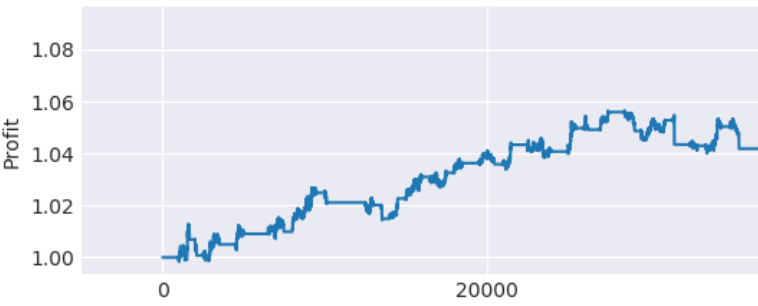
\includegraphics[scale=0.5]{images/stop_loss}
\caption{Exemple de l'effet d'un \textit{trailing stop loss}.}
\end{figure}

\paragraph{}
Nous remarquons dans l'exemple qu'il n'y a pas de grande perte et qu'une perte est souvent suivie d'une période plate. L'application d'un \textit{stop loss}
peut diminuer les pertes et surtout il empêche des comportements humains problématiques. En effet, il arrive qu'une personne prenne une position, que
cette dernière commence à lui faire perdre de l'argent, mais qu'il la garde ouverte en espérant que les choses vont changer et s'améliorer. Le \textit{stop loss}
automatise et empêche ce biais cognitif. Néanmoins cela peut causer d'autres soucis. Lorsqu'une grande baisse survient, le cour descend,
déclenchant le \textit{stop loss}, ce qui va revenir à fermer la position et si de nombreux algorithmes réagissent comme cela, le cour va 
continuer de descendre à cause de la vente simultanée de nombreuses positions créant ainsi un cercle vicieux.

Dans le cadre de notre algorithme, le pourcentage de perte à ne pas dépasser est quantifié par la formule suivante :
$$loss < x * 0.0001$$
Les pertes doivent être plus faibles que $x$ points de bases. Il faut optimiser $x$, car si sa valeur est trop grande, il n'aura aucun effet sur le profit
cumulé. Dans le cas contraire, il deviendra presque impossible de faire du profit, car à la moindre perte, le système va bloquer une position qui aurait pu
engendrer des gains à terme, de plus cela va encourager le système à changer dès que le \textit{stop loss} est déclenché entraînant ainsi une augmentation des
coûts de transactions.

\subsubsection{Implémentation \textit{Layer 2}}
\paragraph{}
L'implémentation du seuil est simple à mettre en place. Le \textit{layer 1} nous renvoie un \texttt{Double}, et il suffit de comparer la valeur avec notre
$y$. Afin de gérer les métas-paramètres ensemble, nous avons créé un objet \texttt{Parameters} qui contient $\delta,\rho,\eta,x,y$. Le pseudo-code
du seuil ressemble à :

\begin{lstlisting}
 ft = computeFt()
 if (math.abs(ft) < param.y) {
  /* traitement du signal */
  }
\end{lstlisting}

Nous avons mentionné le fait qu'il ait plusieurs manières de traiter le signal lorsqu'il est trop faible. Nous avons fait le choix de
retourner :
\begin{lstlisting}
 ft = computeFt()
 if (math.abs(ft) < param.y) {
  ft = 0.0
  }
\end{lstlisting}
De cette manière, en accord avec les équations, cela signifie que nous fermons la position courante. Cela reste cohérent car nous avons
toujours un coût de transaction :
$$ \delta |F_t - F_{t-1}| = \delta (1 - 0)$$
Et nous perdons rien car :
$$ F_{t-1} r_t - \delta | F_t - F_{t-1}| = 0 - \delta | F_t - 0 |$$

\paragraph{}
Concernant le \textit{stop loss}, nous avons créé un objet \texttt{Position}, qui va mémoriser la dernière position ainsi que le profit
cumulé. À partir de cela, voici à quoi ressemble l'implémentation :
\begin{lstlisting}
    ft = computeFt()
 // if we change the position we need to update the max pnl and the position
    if (ft != position.lastPosition) {
        position.maxPnl = position.currentPnl
        position.lastPosition = ft
        return ft
    } else {
        // else we need to check the diff
        val diff = position.maxPnl - position.currentPnl
        if (diff <= 0.0) {
            position.maxPnl = position.currentPnl
        } else if (diff > 0.0 && diff > params.x * 0.001) {
            res = Math.signum(0.0)
        }
    }
\end{lstlisting}

Dans la première partie, nous vérifions que la position est la même. Si ce n'est pas le cas, nous avons juste besoin de mettre à jour la nouvelle
position et le profit cumulé maximum. Sinon, il convient de vérifier.

Si le profit cumulé a augmenté, nous mettons à jours. Et dans le cas contraire, nous vérifions et appliquons le seuil avec $x * 10^{-4}$.
À l'instar, du seuil, nous avons choisi de renvoyer un signal neutre, pour les mêmes raisons mathématiques qu'énoncées plus haut.

\subsubsection{Algorithme \textit{Layer 3}}
\paragraph{}
Cette dernière couche a pour but d'optimiser les métas-paramètres présents dans les couches inférieures. Cela empêche de devoir recourir à une intervention
humaine pour trouver les meilleures valeurs possibles. C'est une solution assez courante dans le domaine du \textit{machine learning}\cite{automated_hyperparamters}. Cette méthode est
souvent opposée à celle de la \textit{grid search} \cite{grid_vs_random}:
\begin{figure}[H]
\centering
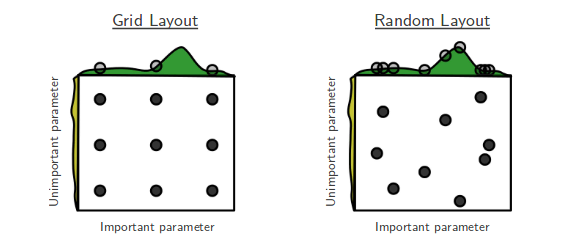
\includegraphics[scale=0.75]{images/grid_vs_random}
\caption{Comparaison entre la méthode d'optimisation \textit{grid search} et celle de \textit{random search}}
\end{figure}

En moyenne, les maximaux locaux sont mieux explorés avec la méthode de recherche aléatoire. Pour mettre en place cet algorithme, il faut définir une
fonction de coût, afin d'évaluer la qualité d'une solution.
Les fonctions qui rentrent en compte sont les suivantes :
\begin{center}
 $$ \Sigma := \frac{\sum_{i=0}^N (R_i)^2 I (R_i < 0)}{\sum_{i=0}^N (R_i)^2 I (R_i > 0)}$$
 $$ U(\bar{R}, \Sigma, \nu) := a (1 - \nu) \bar{R} - \nu \Sigma$$
\end{center}

Où $\bar{R} := \frac{P_N}{N}$ est le profit moyen avec $N$ le nombre d'éléments, $\nu$ l'aversion au risque et $a$ est une constante.
Dans la formule $\Sigma$, intuitivement on comprend que l'on veut un maximum de $R_i > 0$ et un minimum de $R_i < 0$, ce qui implique que la valeur
optimale de cette formule vaut $0$. Ceci est confirmé dans la deuxième formule $U$. En effet, on va soustraire $\nu \Sigma$, donc si $\Sigma$ vaut $0$,
on maximise la fonction de coût. De plus $\bar{R}$ est défini comme le profit moyen, plus il sera grand, plus $U$ sera grand.

La direction optimale à suivre est celle qui va maximiser les profits positifs tout en minimisant les profits négatifs, ce qui est intuitif.
L'article mentionne d'autres raisons qui appuient ce choix \cite{fx_trading}:
\begin{enumerate}
 \item Les stratégies avec un grand risque et de nombreux \textit{returns} négatifs sont pénalisés dans la définition de $\Sigma$.
 \item Le fait de construire $\Sigma$ comme un ratio permet d'obtenir des résultats similaires même si le volume augmente. Par exemple, pour une même
 stratégie qui serait stable, si l'on calcule avec 1'000 ou avec 1'000'000, le ratio serait similaire\footnote{De part notre hypothèse d'une stratégie stable}.
\end{enumerate}

Le but étant de maximiser $U$, la fonction de coût devient :
$$\max\limits_{\delta, \eta, \rho, x, y} U(\bar{R};\Sigma : \delta, \eta, \rho, x, y; \nu)$$

Avec, pour rappel, $\delta$ le coût de transaction, $\eta$ le paramètre d'adaptation, $\rho$ le paramètre d'apprentissage, $x$ le \textit{stop trailling
loss} et $y$ le seuil. Malheureusement, cette fonction est trop complexe pour être optimisé de manière analytique. Il faut recourir à des heuristiques.
L'article en propose une qui s'exprime sous cette forme :
$$\max\limits_{\delta} \max\limits_{\eta} \max\limits_{\rho} \max\limits_{x} \max\limits_{y} U(\bar{R};\Sigma : \delta, \eta, \rho, x, y; \nu)$$

Il s'agît d'une recherche aléatoire composante par composante. Ils fixent quatre paramètres puis ils tirent 15 valeurs aléatoires normalement distribuées
autour de la valeur initiale, puis ils évaluent la fonction pour chacune des 15 valeurs et prennent la meilleure. Puis l'optimisation reprend avec le 
paramètre suivant. C'est une formule assez simple, qui a le mérite d'être peu coûteuse en ressources de calculs.

\paragraph{}
Comme pour le \textit{Layer 2}, l'implémentation du \textit{Layer 3} reprend fidèlement les équations proposées. Voici la manière dont fonctionne
l'optimisation :
\begin{enumerate}
 \item Nous sélectionnons un intervalle de \textit{returns}.
 \item Nous fixons 4 paramètres parmi les 5.
 \item Nous tirons une valeur aléatoire normalement distribuée centrée sur la valeur initiale.
 \item Pour tout l'intervalle, nous lançons le \textit{Layer 1 \& 2} avec les métas-paramètres.
 \item Nous récupérons les valeurs importantes et nous calculons $U(\bar{R};\Sigma : \delta, \eta, \rho, x, y; \nu)$.
 \item Nous stockons le résultat.
 \item Si nous avons terminé les 15 tirages, nous fixons la nouvelle valeur du paramètre avec le meilleur résultat\footnote{i.e: la meilleure valeur de 
 $U(\bar{R};\Sigma : \delta, \eta, \rho, x, y; \nu)$ parmi celles stockées du point 6.} et retournons au point 2. Sinon nous reprenons au point 3.
\end{enumerate}

Une fois que les cinq paramètres ont été optimisés, nous pouvons mettre à jour les nouveaux paramètres et reprendre l'entraînement du \textit{Layer 1}.
Les paramètres ont initialement une valeur aléatoire $\in [0,1]$ car nous n'avons aucune indication sur leur valeur optimale. Nous avons donc choisi d'utiliser une distribution gaussienne :
$$\mathcal{N}(\mu,\sigma)$$

Où, $\mu$ est égale à la valeur initiale du paramètre et $\sigma = 1$. Ce sont des valeurs arbitraires. Nous estimons que chercher des valeurs avec une déviation
standard de 1 permet d'explorer l'espace tout en évitant d'avoir des changements trop brutaux.

\subsubsection{Implémentation \textit{Layer 3}}
\paragraph{}
Dans l'implémentation, les paramètres sont réunis dans une classe et c'est cette classe qui dispose des méthodes pour optimiser et mettre à 
jour les valeurs. De plus, par le caractère décorrélé des calculs pour les 15 tirages aléatoires, nous avons construit cela avec des \textit{Thread}. Cela
permet d'avoir de meilleur performance, car avec un \textit{Pool} gérant les cœurs disponibles, on lance un \textit{Thread} par valeur, pour un 
paramètre donné, et il suffit juste de synchroniser le moment
où les \textit{Thread} auront terminé et de prendre le meilleur résultat. De part le peu de synchronisation nécessaire, cela ne crée pas de perte de
performance. Il est donc possible de gagner un facteur $fac$ plus ou moins équivalent au nombre de cœurs engagés dans le calcul.

Afin de donner une idée du gain, utilisons des valeurs fictives. Soit le calcul pour un jeu de valeur $t$ qui vaut $1$, la comparaison afin de trouver la meilleur valeur $comp$ vaut $0.5$.
Pour $m$ paramètres et $n$ tirages, cela donne dans notre cas $m=5$ et $n=15$:
$$m n (t + comp) = 5 * 15 * (1 + 0.5) = 112.5$$

Imaginons maintenant l'exemple avec $processus=4$ en parallèles. Cela nous donne :
$$ \frac{m n}{processus} (t + comp) + \epsilon = \frac{5 * 15}{4} * (1 + 0.5) = 28.125$$
Où $\epsilon$ est notre mécanisme de synchronisation, ce dernier reste négligeable de part la nature décorrélée des calculs.
Le gain est très important tout en étant facilement \textit{scalable}. En effet, l'ordonnancement des tâches est opéré par la machine virtuelle Java, ce sont donc des considérations hauts niveaux ne nécessitant pas de grande connaissances en parallélisme.

\subsubsection{Points problématiques}
\paragraph{}
Durant l'implémentation, nous nous sommes trouvés confrontés à plusieurs problèmes algorithmiques. Dans cette section, nous allons les détailler et présenter les solutions appliquées ou envisagées.

\paragraph{}
Le principal problème, qui nous empêche d'obtenir des résultats, est que les poids du réseau de neurones divergent durant la descente du gradient.
Au bout de quelques centaines d'itérations, les poids croissent rapidement et deviennent tous \texttt{NaN}. Voici deux exemples de \textit{runs} afin de
montrer le comportement des poids :
\begin{figure}[H]
\centering
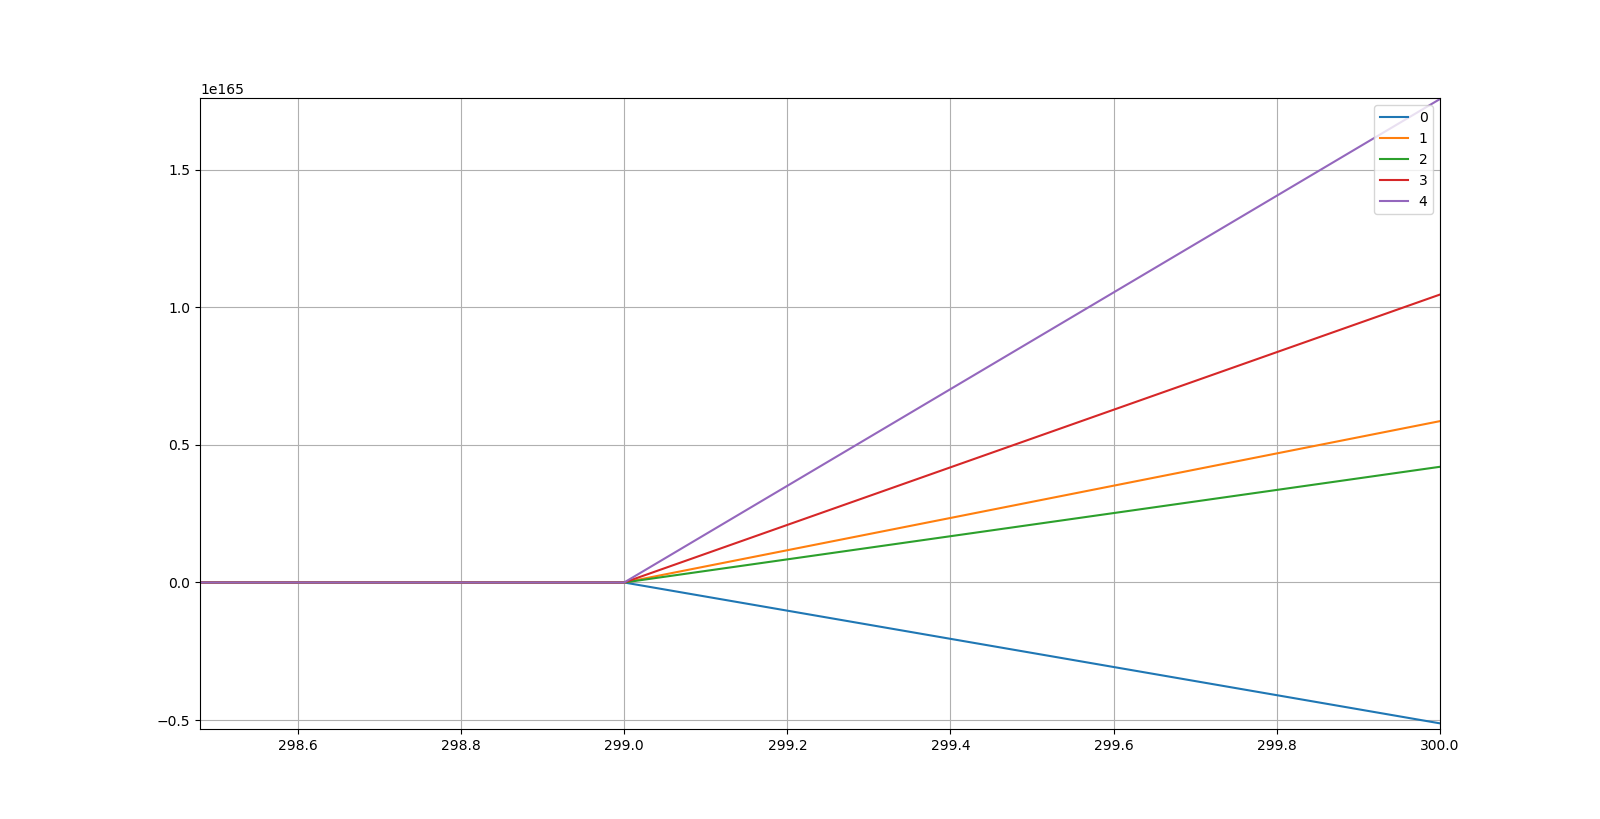
\includegraphics[scale=0.40]{images/run_1}
\caption{Exemple de la divergence des valeurs des poids pour une \textit{run} standard de l'algorithme, où l'axe des abscisses représente l'itération et
l'axe des ordonnées la valeur.}
\end{figure}

\begin{figure}[H]
\centering
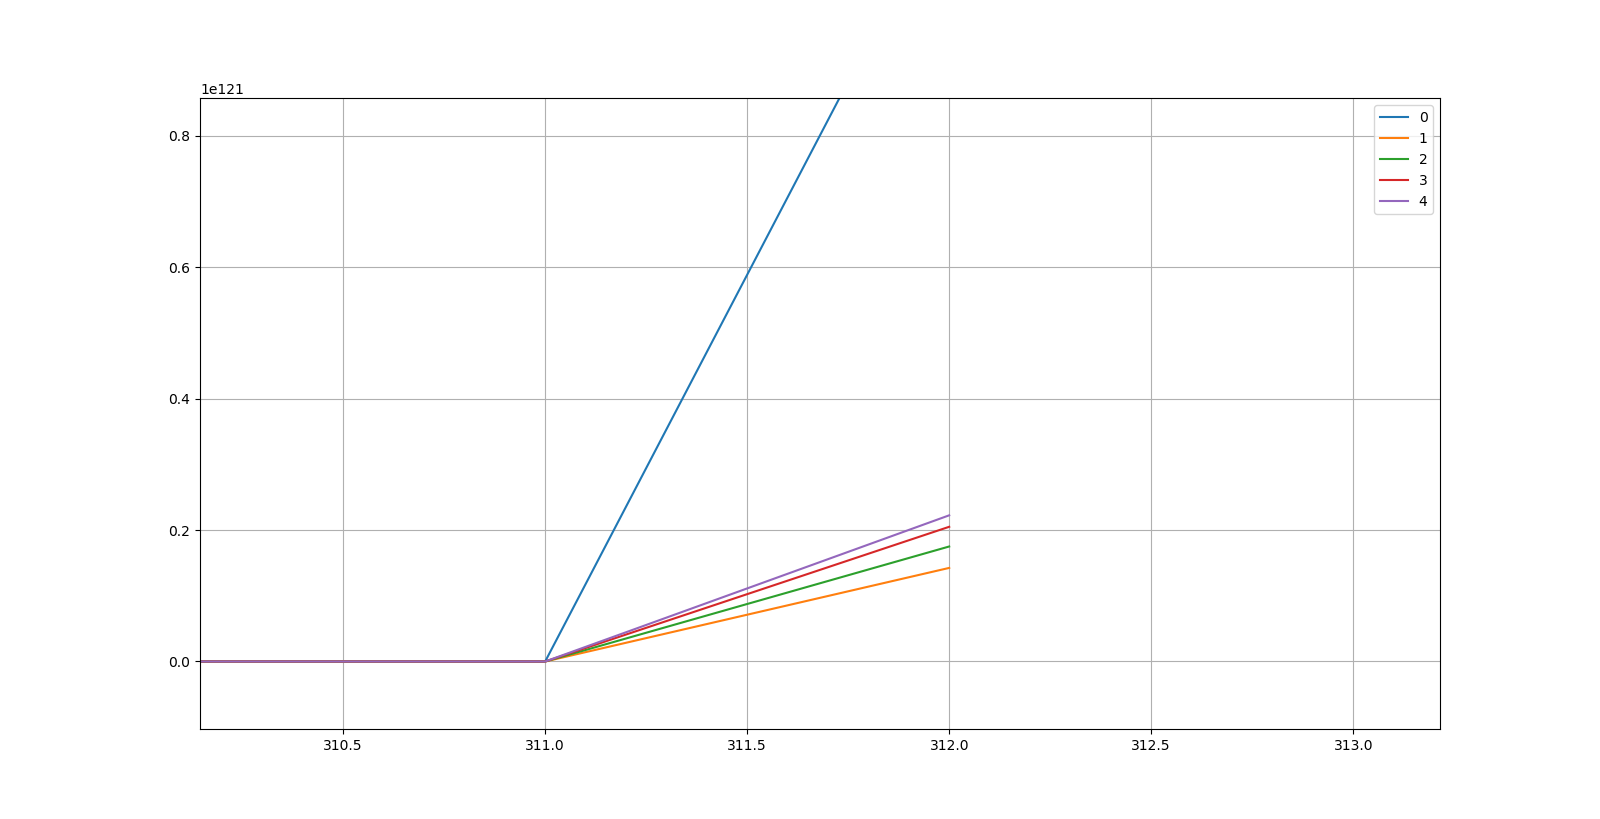
\includegraphics[scale=0.4]{images/run_2}
\caption{Autre exemple de la divergence des valeurs des poids pour une \textit{run} standard de l'algorithme.}
\end{figure}

Ce phénomène peut avoir pour cause un \textit{learning rate}\footnote{Dans notre cas, il s'agît de $\rho$.} trop grand. En effet, si ce dernier a une
valeur trop importante, à chaque itération la valeur risque de croître et donc de diverger. Une solution intuitive consisterait à diminuer le taux afin
d'éviter cela. Nous avons donc tenté cette méthode qui s'est révélée être infructueuse. Pour toutes les valeurs testées, pour la plupart comprises
dans $ [10^{-5},10^{-2}]$, l'algorithme avait deux comportements\footnote{Les valeurs sont indicatives mais cela peut varier.}:
\begin{itemize}
 \item Pour les valeurs plus petites que $10^{-3}$, le taux d'apprentissage était trop faible et les valeurs des poids ne changeaient pas.
 \item Pour les valeurs plus grandes que $10^{-3}$, nous retrouvions un comportement divergeant.
\end{itemize}

L'article faisait mention d'un facteur $f < 1$ permettant d'éviter ces problèmes \cite{fx_trading}. Il est possible de multiplier les poids, lorsqu'il 
dépasse une certaine valeur par le dît facteur, afin d'endiguer une croissance trop rapide. Le pseudo-code correspondant ressemble à cela :
\begin{lstlisting}
 for weight in weights
     if abs(weight) > some_threashold
         weight = weight * f
     endif
 endfor
\end{lstlisting}

Ici encore, il y a un choix à faire sur la valeur de $f$, nous avons donc testé pour plusieurs cas. Il ressort deux cas de figures :
\begin{itemize}
 \item Si $f$ a une valeur trop petite, alors les poids n'ont pas le temps de croître. Ils auront donc tendance à stagner ou à tendre vers $0$.
 \item Dans le cas contraire, la multiplication ne fait pas assez diminuer la valeur des poids et ils tendent toujours vers l'infini.
\end{itemize}

Nous avons également tenté de combiner ces deux techniques en espérant que leur application conjointes permettent d'éviter ces problèmes, mais les
résultats n'ont pas changé des situations mentionnées précédemment.
\paragraph{}
En essayant d'autres outils afin de voir si le problème persiste, nous nous sommes rendus compte qu'en utilisant une bibliothèque reconnue de réseaux de 
neurones\cite{keras}, cette divergence existait également. Donc pour des données similaires, avec un algorithme d'optimisation similaire mais un réseau de neurones
différent et une fonction de coût différente, nous arrivons au même problème.
Nous sommes donc parti de l'hypothèse que le problème se trouvait dans la méthode d'optimisation, soit la descente du gradient. En changeant de méthode
dans la bibliothèque, nous avons obtenu des résultats\footnote{i.e: Les valeurs des poids ne divergeaient plus.} plutôt bon.

Les algorithmes ayant données satisfactions sont \cite{keras}:
\begin{itemize}
 \item Adagrad.
 \item Adadelta.
 \item RMSProp.
\end{itemize}

  Nous avons donc lu la documentation et les publications afin de comprendre le fonctionnement de ces algorithmes. Et \textit{in fine}, trouver les 
  différences avec la descente du gradient qui pourraient expliquer les écarts de résultats.
  
  En lisant les sources des algorithmes sus-mentionnés, nous nous sommes rendus compte de deux éléments très importants. Il s'agît de variantes de la
  descente du gradient et surtout, ils ont pour point commun d'avoir un taux d'apprentissage variable.
  
  En effet, dans la descente du gradient, le taux d'apprentissage est fixé pour une \textit{run} donnée, ce qui nous a posé les problèmes expliqués précédemment.
  Pour ces algorithmes, le taux d'apprentissage est modifié à chaque itération d'une \textit{run} permettant plus de flexibilité, un apprentissage plus 
  rapide et de diminuer le risque de divergence.
  \begin{itemize}
   \item Pour le RMSProp, il faut diviser le taux d'apprentissage par la moyenne des magnitudes des précédents gradients pour chaque poids \cite{rmsprop}.
   \item L'article sur l'Adadelta mentionne le fait que si l'on utilise \cite{adadelta}:
   $$\Delta x_t = H_t^{-1}g_t$$
   où $H_t^{-1}$ est l'inverse de la matrice Hessienne et $g_t$ le gradient, à l'itération $t$. Cela donne le poids optimal pour des problèmes quadratiques.
   Le coût de calcul étant trop important, l'article montre comment approximer cela en utilisant des heuristiques.
   \item Pour l'algorithme Adagrad, le taux d'apprentissage est calculé à partir des paramètres.
  \end{itemize}

  Il nous a semblé que l'algorithme RMSProp était le plus simple à mettre en place. Nous avons donc appliqué les formules suivantes \cite{rmsprop_algo} :
  $$E[g^2]_t = 0.9 E[g^2]_{t-1} + 0.1 g^2_t$$
  où $g$ est le gradient et $E[g^2]_t$ l'espérance du carré du gradient au temps $t$. À partir de cela :
  $$\theta_{t+1} = \theta_t + \frac{\rho}{\sqrt{E[g^2]_t + \epsilon}} g_t$$
  Nous avons donc un taux d'apprentissage qui varie en fonction des résultats précédemment obtenus, ce qui pourrait résoudre le problème rencontré avec la
  descente du gradient dans sa version simple.
  
  Après avoir implémenté, cet algorithme, nous nous retrouvions également avec des poids qui divergeaient. En effet, de part les facteurs $0.9$ et $0.1$ 
  le soucis persistait car l'espérance $E[g^2]_t$ n'était pas suffisamment grande pour compenser la croissance des poids. Nous avons donc changé les 
  coefficients et testé plusieurs combinaisons. Nous avons obtenu de bons résultats avec $1$ et $0.1$ :
  $$E[g^2]_t = E[g^2]_{t-1} + 0.1 g^2_t$$
  
  La partie intéressante de cette méthode est la manière dont elle accélère l'apprentissage. En effet, si $E[g^2]_t < 1$, on a des changements minimes 
  qui risquent de prendre du temps pour converger\footnote{Avec la version classique de la descente du gradient.}. Cependant en divisant $\rho$ par ce
  nombre, on va augmenter la "quantité de changement" rendant la convergence plus rapide. À contrario, si $E[g^2]_t > 1$, nous avons des changements 
  conséquents et donc un risque de divergence\footnote{Également avec la version classique de la descente du gradient.}. Pour éviter cela, par la division,
  nous diminuons l'impact de ces modifications, diminuant \textit{de facto} le risque de divergence.
  
  \paragraph{}
  Nous supposons, pour ce paragraphe, être dans un état où la descente du gradient et le \textit{Layer 2} fonctionnent. Nous nous intéressons donc à la couche 
  d'optimisation des métas-paramètres\footnote{Aussi noté hyperparamètres dans la littérature.}. La liste de ces derniers est la suivante :
  \begin{itemize}
   \item $\rho$ le taux d'apprentissage.
   \item $\eta$ le paramètre d'adaptation.
   \item $\delta$ le coût de transaction.
   \item $x$ le \textit{trailing stop loss}.
   \item $y$ le seuil.
  \end{itemize}

  Comme mentionné précédemment, l'optimisation de $\rho$ perd de son intérêt de par l'utilisation de l'algorithme RMSProp conjointement à la descente du
  gradient. De plus, il paraît étonnant d'optimiser le coût de transaction $\delta$. Cette valeur ne dépend pas d'un processus d'optimisation, il est
  étrange de vouloir la modifier.
  
  À partir de là, nous allons travailler uniquement sur $\eta,x,$ et $y$. En utilisant l'algorithme présenté plus haut, nous avons eu des problèmes
  de signal nul ou de \texttt{NaN}. Cela peut varier d'une \textit{run} à l'autre. Ces phénomènes arrivent car dans le premier cas le seuil et/ou le \textit{stop
  loss} sont trop élevés ne laissant aucun signal être accepté, et dans le second cas, les valeurs sont également trop grande, car qui provoque des erreurs
  de calculs en chaîne entraînant des poids divergeant malgré l'algorithme du RMSProp.
  
  Pour palier ce problème pour $t=0$, nous avons fixé les valeurs initiales plutôt que d'utiliser un tirage aléatoire. Pour $t>0$ cependant, il
  faut modifier la déviation standard. Cette dernière, si la valeur est trop grande, risque de faire diverger les résultats de l'optimum.
  Les nouvelles valeurs des paramètres sont calculées de manière aléatoire suivant une distribution gaussienne:
  $$x_{t+1} = \mathcal{N}(\mu, \sigma)$$
  où $\mu = x_t$ et $\sigma$ est initialisé à $\mu/10 + \epsilon$ afin d'éviter des sauts trop rapides. Cela permet d'explorer l'espace sans risquer de
  sortir de la zone d'attraction de l'optimum.
 
 Nous soupçonnons le fait que les paramètres $\eta$ et $\delta$ ont un impact trop grand dans le calcul de $A_t$ et $B_t$ ce qui pouvait entraîner les
 problèmes de poids. Pour éviter cela, nous avons fixé une valeur très faible, de l'ordre de $10^{-3}$, ce qui fait disparaître le problème.
 De plus, malgré l'optimisation, les meilleurs résultats en moyenne sont obtenus avec les valeurs initiales pour $x$ et $y$. Ces paramètres, lorsque 
 $x$ devient grand et $y$ petit n'ont que peu d'influence sur la fonction de coût et donc il est compliqué de trouver de meilleures valeurs.
 De plus, nous ne connaissons pas le domaine dans lequel chercher les solutions ce qui handicape grandement la recherche. Si la déviation standard est trop importante cela fait diverger les valeurs et nous obtenons de très mauvais résultats\footnote{i.e: Un profit cumulé pouvant atteindre des valeurs aberrante comme des pertes de l'ordre de 100 unités.} et si elle est trop petite, nous restons dans
 la zone d'attraction de la moyenne ce qui retire tout l'intérêt de l'optimisation.
 Nous n'avons pas de solution pour cette partie et il conviendrait de chercher une solution dans des recherches futures.
 

\paragraph{}
Afin de donner une vision d'ensemble, voici un pseudo-code résumant le schéma global du programme :
  \begin{lstlisting}
 // initialization part
 delta, rho, eta, x, y = Random()
 weights = Random()
 F[0] = 0		// the vector of signal
 t = 1			// the time
 oldPrice = prices[0]	// the current prices
 returns[0] = 0		// init the vector of return
 
 // training phase with 2000 steps
 for price in prices[1:2001]:
 	// computing the return
 	r = price - oldPrice
 	oldPrice = price
 	returns[t] = r
 	// compute the signal
 	F[t] = computedFt(t, w, F[t-1], returns, x, y)
 	// update the weights
 	w = updateWeights(returns[t-1], F[t-1], F[t], delta, rho, eta, x, y, returns)
 	// recompute the F[t] with new best weights
 	F[t] = computedFt(t, w, F[t-1], returns, x, y)
 	// if we reach the time to update parameters
 	if (t % 500 == 0):
 		delta, rho, eta, x, y = updateParameters(returns, w)
 	t++
 
 // for the testing phase, or the production phase
 t = 1
 pnl[0] = 0
 // clean returns and F
 F[0] = 0
 returns[0] = 0
 // the loop with index right after the training phase
 for price in prices[2001:2501]:
 	r = price - oldPrice
 	oldPrice = price
 	returns[t] = r
 	F[t] = computedFt(t, w, F[t-1], returns, x, y)
 	pnl[t] = pnl[t-1] + (F[t-1] * returns[t-1] - delta * |F[t-1] - F[t]|)
 
 return pnl
  \end{lstlisting}
 
\subsubsection{Résultats}
 \paragraph{}
 Afin de faciliter la comparaison avec l'article sur lequel est basé notre projet,nous allons utiliser les mêmes données. À savoir le cours EURUSD de Janvier 2000 à Janvier 2002. La granularité des données est de une mesure tout les minutes.
 
 \todo[inline]{Ajouter graphique p\&l + cours. Plus blabla sur la comparaison.}
 
 \paragraph{}
 Malheureusement l'approche scientifique de l'article est bancal. En effet, les résultats présentés ne sont basés sur que un unique jeu de données et sur une seule période. Il n'est donc pas évident d'analyser si les résultats proviennent de la qualité intrinsèque de l'algorithme ou du fait qu'il s'agisse "d'une bonne période". Pour pallier cela, nous avons approfondi les mesures en prenant d'autres périodes, d'autres paires de monnaies ainsi que des fenêtres d'apprentissages différentes.
 
 Dans un premier temps, voici des tests sur le même cours, soit l'EUR/USD, mais sur l'année 2004.
 Les graphiques présentent trois éléments :
 \begin{enumerate}
  \item Le cours de change afin de visualiser la tendance.
  \item Le signal. Cela permet de voir si le signal correspond à la tendance du cours ou de voir si le signal est nul.
  \item Le profit cumulé.
 \end{enumerate}

Afin de mieux discerner les éléments importants, nous avons décomposer les  données en cinq graphiques différents, rendant l'ensemble plus lisible.
 
 \begin{sidewaysfigure}
\centering
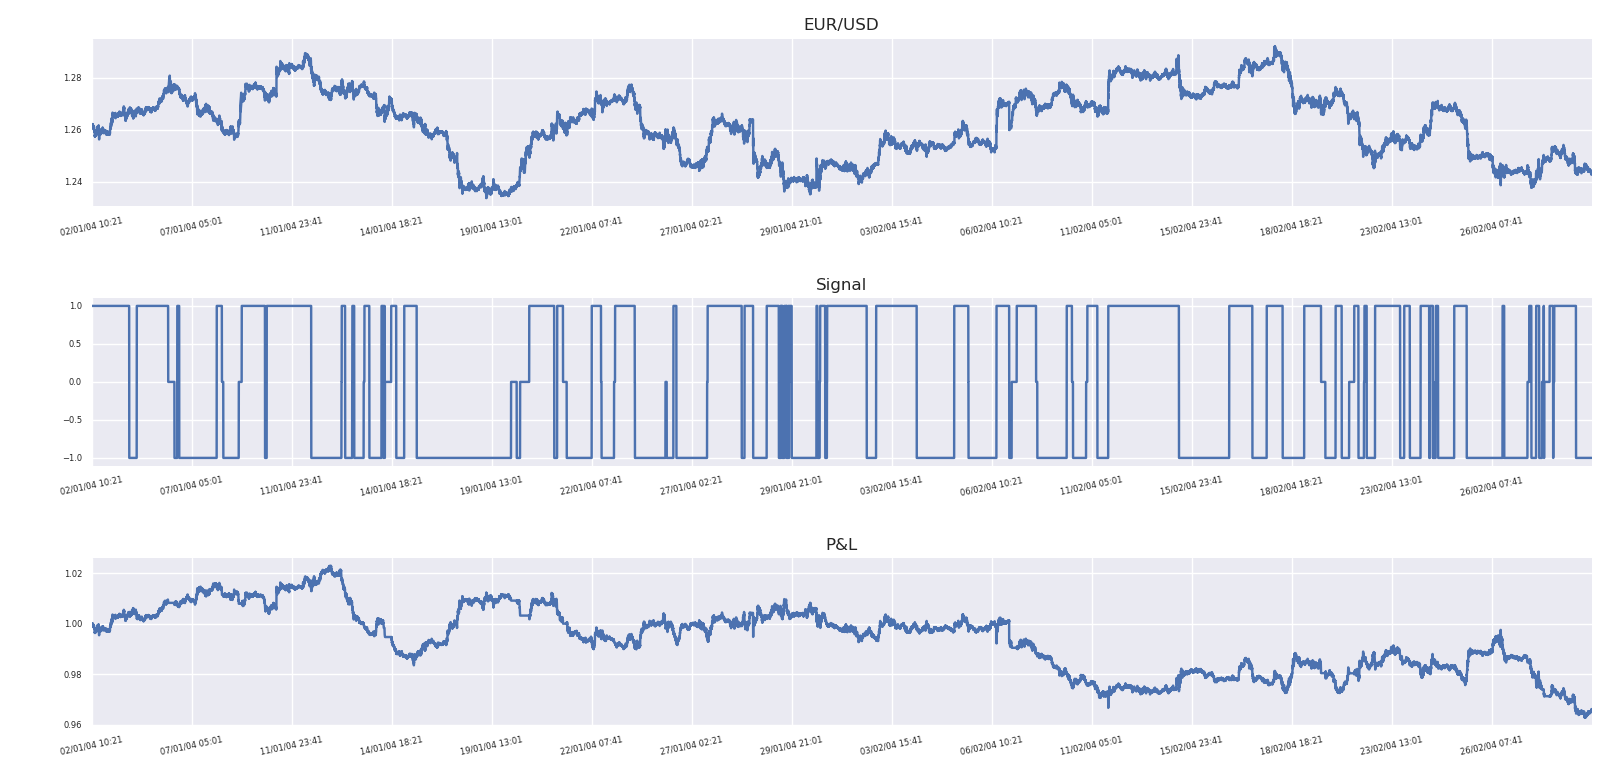
\includegraphics[scale=0.5]{res/eursud_2004-2005_from_0to_10000}
\caption[Blup]{Cours EUR/USD entre le 01.01.2004 et le 01.01.2005, avec $|w| = 20$, $2000$ éléments d'entraînement, $500$ de test, une optimisation des
paramètres toutes les $200$ itérations durant la phase d'apprentissage, $\delta = 0.001, \eta=0.001,\rho=0.01$
\footnotemark$, x = 0.005, y=0.0001$.}
\end{sidewaysfigure}
\footnotetext{Valeur de $\rho$ avant l'optimisation par RMSProp}

 \begin{sidewaysfigure}
\centering
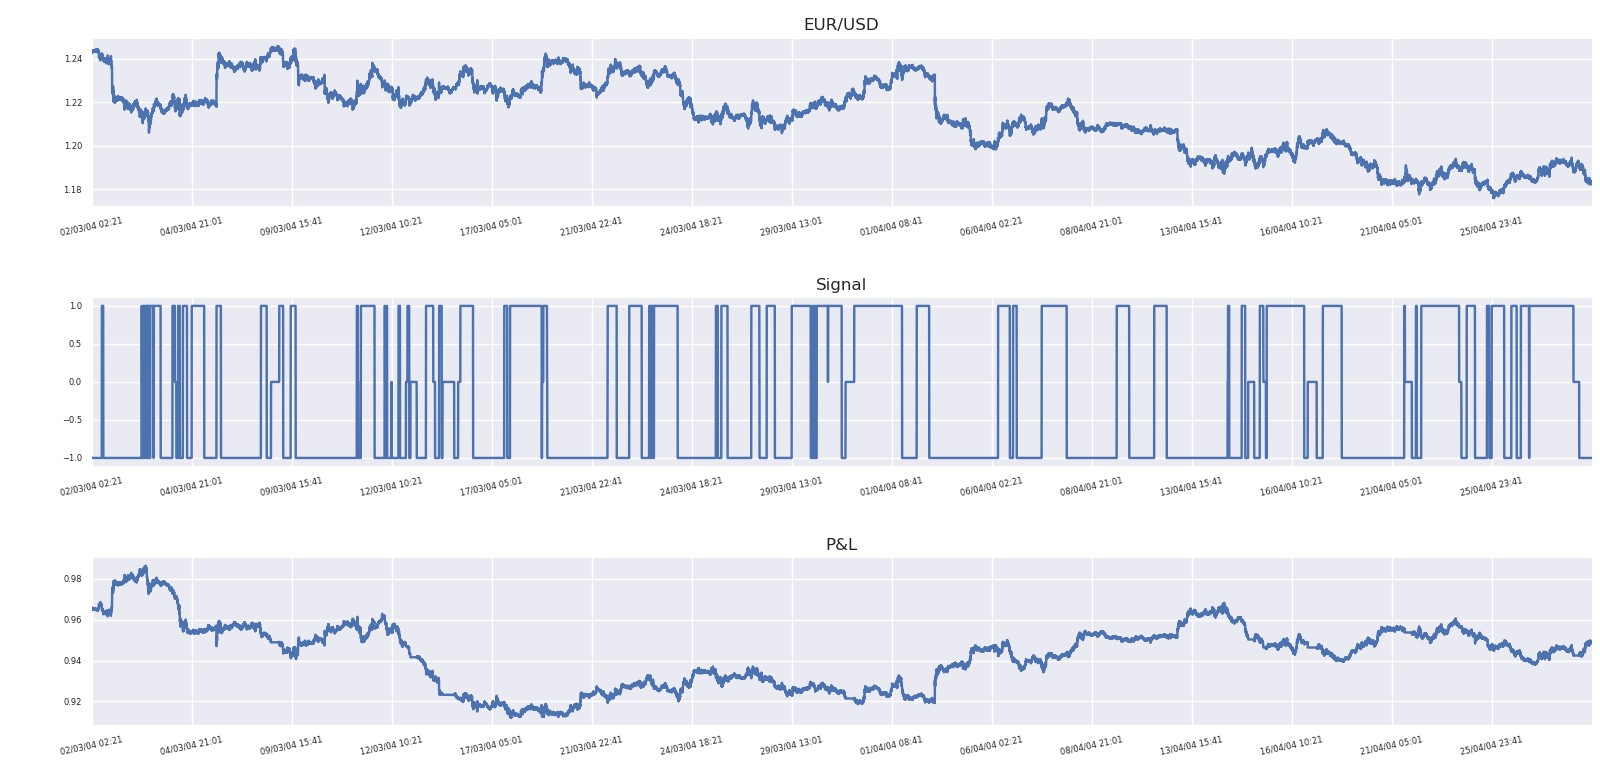
\includegraphics[scale=0.5]{res/eursud_2004-2005_from_10000to_20000}
\caption[Blup]{Cours EUR/USD entre le 01.01.2004 et le 01.01.2005, avec $|w| = 20$, $2000$ éléments d'entraînement, $500$ de test, une optimisation des
	paramètres toutes les $200$ itérations durant la phase d'apprentissage, $\delta = 0.001, \eta=0.001,\rho=0.01, x = 0.005, y=0.0001$.}
\end{sidewaysfigure}

 \begin{sidewaysfigure}
	\centering
	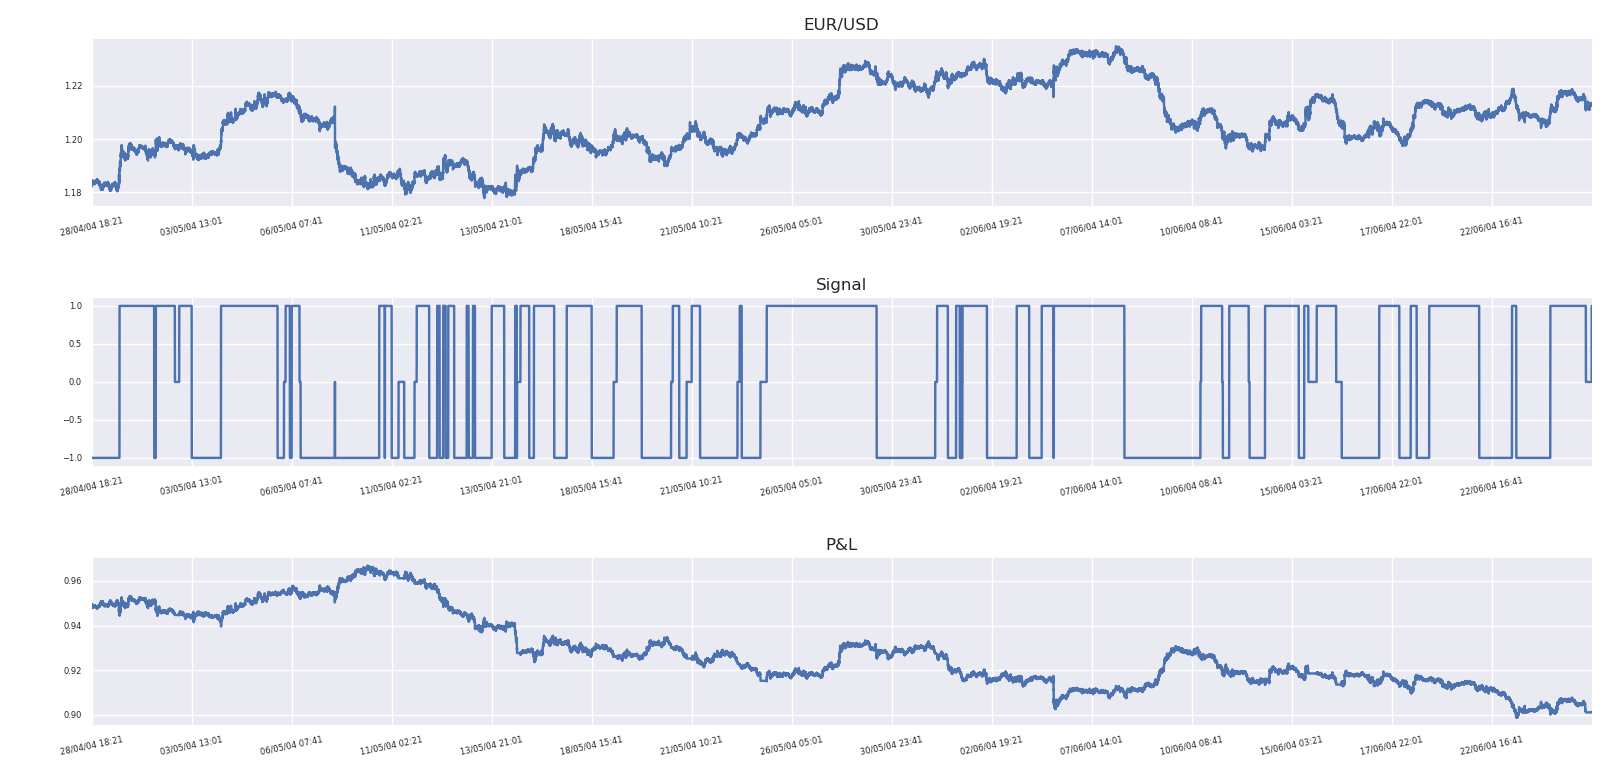
\includegraphics[scale=0.5]{res/eursud_2004-2005_from_20000to_30000}
	\caption[Blup]{Cours EUR/USD entre le 01.01.2004 et le 01.01.2005, avec $|w| = 20$, $2000$ éléments d'entraînement, $500$ de test, une optimisation des
		paramètres toutes les $200$ itérations durant la phase d'apprentissage, $\delta = 0.001, \eta=0.001,\rho=0.01, x = 0.005, y=0.0001$.}
\end{sidewaysfigure}

 \begin{sidewaysfigure}
	\centering
	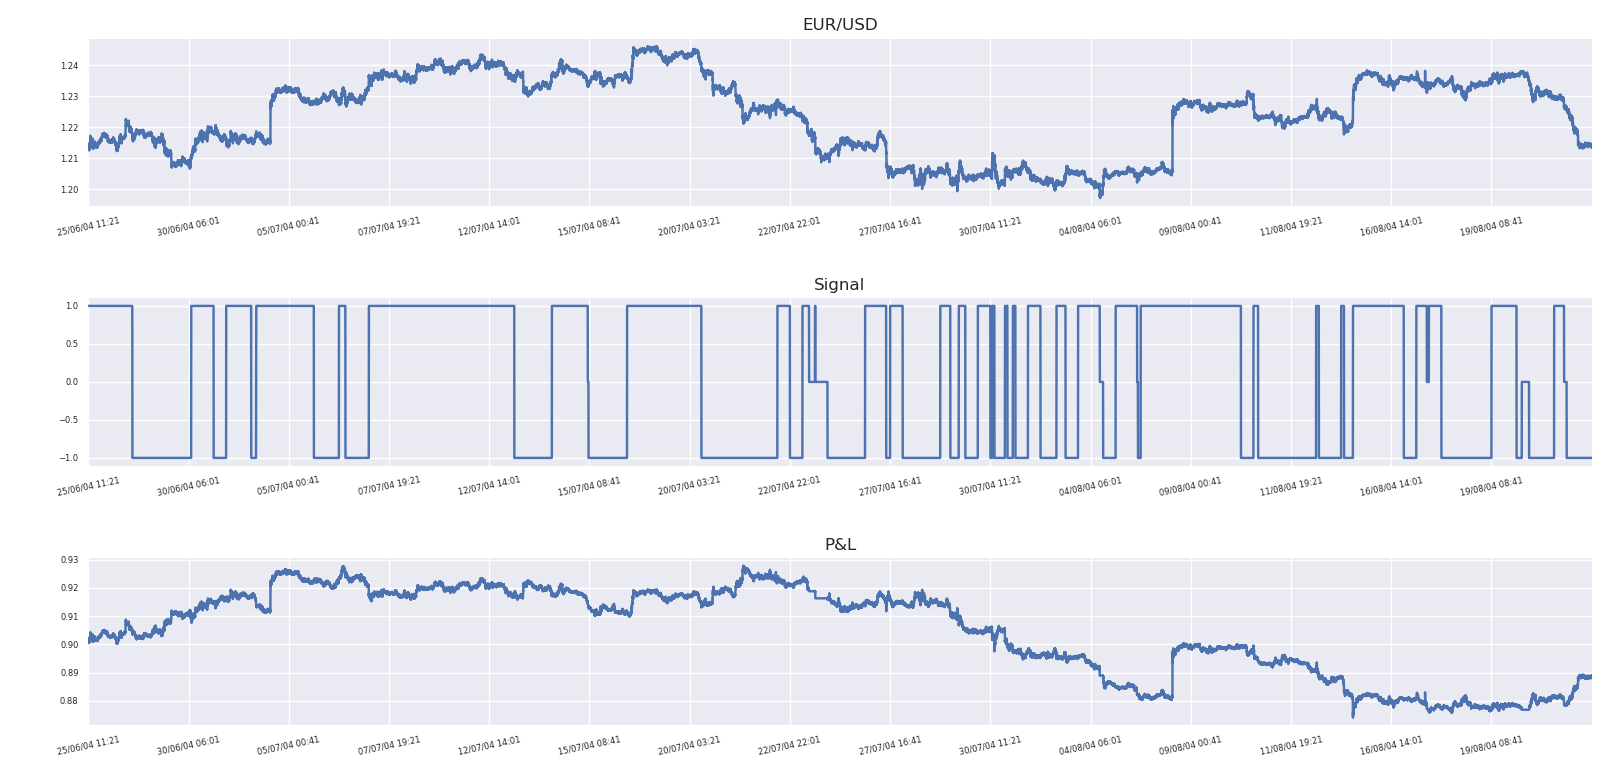
\includegraphics[scale=0.5]{res/eursud_2004-2005_from_30000to_40000}
	\caption[Blup]{Cours EUR/USD entre le 01.01.2004 et le 01.01.2005, avec $|w| = 20$, $2000$ éléments d'entraînement, $500$ de test, une optimisation des
		paramètres toutes les $200$ itérations durant la phase d'apprentissage, $\delta = 0.001, \eta=0.001,\rho=0.01, x = 0.005, y=0.0001$.}
\end{sidewaysfigure}

 \begin{sidewaysfigure}
	\centering
	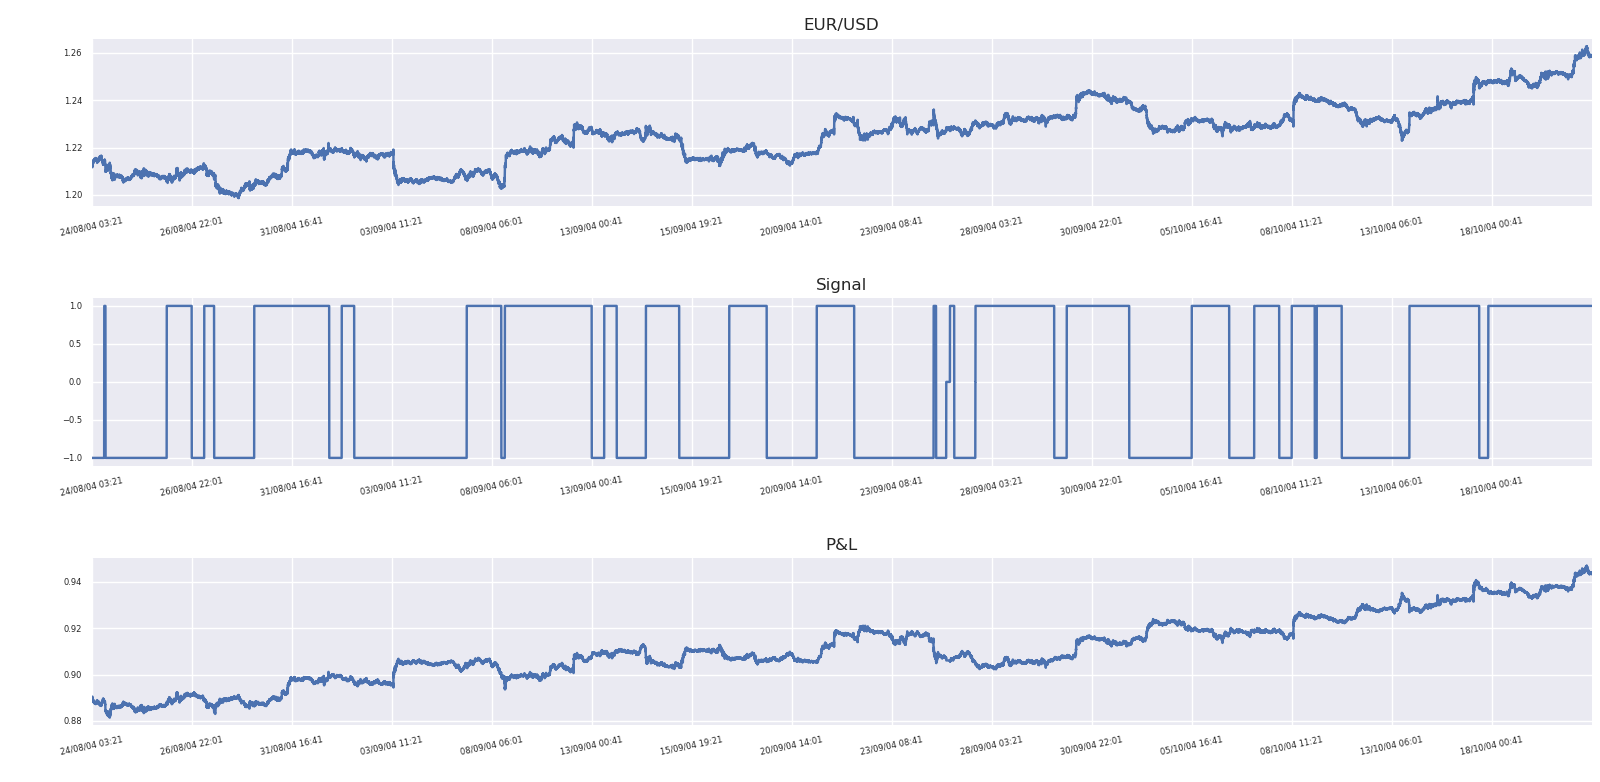
\includegraphics[scale=0.5]{res/eursud_2004-2005_from_40000to_50000}
	\caption[Blup]{Cours EUR/USD entre le 01.01.2004 et le 01.01.2005, avec $|w| = 20$, $2000$ éléments d'entraînement, $500$ de test, une optimisation des
		paramètres toutes les $200$ itérations durant la phase d'apprentissage, $\delta = 0.001, \eta=0.001,\rho=0.01, x = 0.005, y=0.0001$.}
\end{sidewaysfigure}


\paragraph{}
Il peut y avoir, entre différentes \textit{runs}, des différences significatives. Nous allons prendre un exemple simple afin d'expliquer l'origine du problème.

De part l'initialisation aléatoire, pour trois poids, nous avons :
\begin{itemize}
	\item Durant la \textit{run} 1, $w_1=0.5,w_2=0.1,w_3=0.1$.
	\item Durant la \textit{run} 2, $w_1=0.1,w_2=0.1,w_3=0.5$.
\end{itemize}

Pour des \textit{returns} valant $r_1=0.3,r_2=-0.1,r_3=-0.4$. Nous avons pour $sign(\sum_{i=1}^{3}w_i * r_i)$:
\begin{itemize}
	\item Pour la \textit{run} 1, $0.5 * 0.3 + 0.1 * -0.1 + 0.1 * -0.4 = 0.1$.
	\item Pour la \textit{run} 2, $0.1 * 0.3 + 0.1 * -0.1 + 0.5 * -0.4 = -0.18$.
\end{itemize}

Ce que nous voulons montrer par cet exemple simple, c'est que pour de mêmes données, soit nos $r_i$, les différences des $w_i$ peuvent entraîner des changements en terme de décision et donc de profit.

De plus, la méthode d'optimisation ne garantit pas de trouver le minimum global. Il est donc fortement possible que les directions d'optimisations ne soient pas pareilles conduisant ainsi à des situations similaires. Afin de trouver des résultats identiques d'une fois à l'autre, il faut fixer l'aléatoire de la classe \textit{Random}.
 
 
 \paragraph{}
 Nous avons voulu observer l'évolution de \textit{Sharpe ratio} pour diverses valeurs de $\eta$, afin de voir si le ratio est optimisé et l'impact
 du paramètre $\eta$ dans ce ratio. Les graphiques suivants sont calculés à partir du cours EUR/CHF entre le 03.01.2010 et le 30.12.2011, avec 
 $|w| = 20$, $2000$ éléments d'entraînement, $500$ de test, une optimisation des
paramètres toute les $200$ itérations durant la phase d'apprentissage, $\delta = 0.001, \rho=0.01, x = 0.005, y=0.0001$. Nous n'avons pris en compte 
les résultats de la première itération d'apprentissage. Soit $t= [0,2000]$.
Pour rappel le \textit{Sharpe ratio} se calcule de la manière suivante :
$$\widehat{S}(t) := \frac{A_t}{B_t}$$
où $A_t := A_{t-1} + \eta (R_t - A_{t-1})$ et $B_t := B_{t-1} + \eta (R_t^2 - B_{t-1})$.


  \begin{figure}[H]
\centering
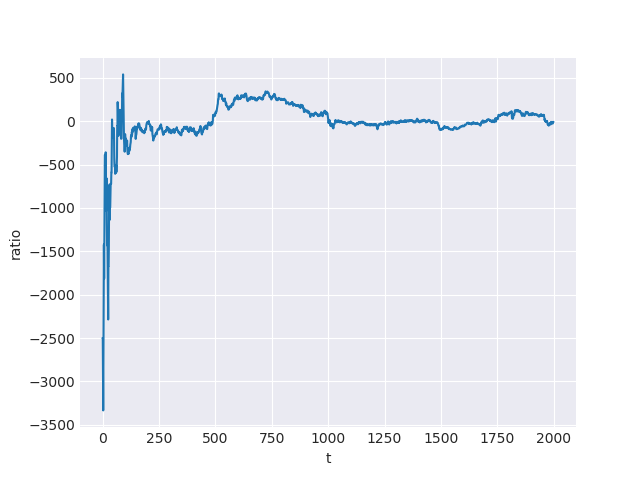
\includegraphics[]{res/exemple_eta_0001}
\caption[Blup]{Évolution du \textit{Sharpe ratio} avec $\eta = 0.001$, $A_0 = 0, B_0 = 0$ de $t=0$ à $t=2000$}
\end{figure}

  \begin{figure}[H]
\centering
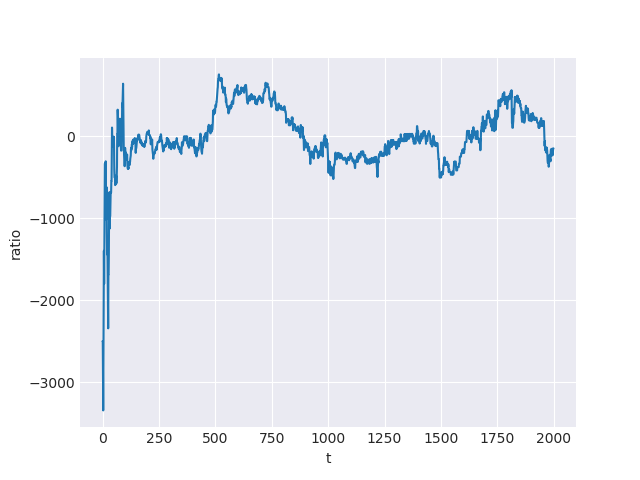
\includegraphics[]{res/exemple_eta_0005}
\caption[Blup]{Évolution du \textit{Sharpe ratio} avec $\eta = 0.005$, $A_0 = 0, B_0 = 0$ de $t=0$ à $t=2000$}
\end{figure}

  \begin{figure}[H]
\centering
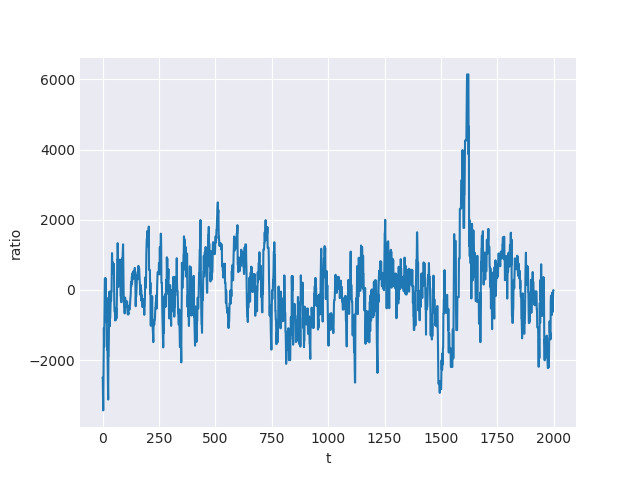
\includegraphics[]{res/exemple_eta_too_big}
\caption[Blup]{Évolution du \textit{Sharpe ratio} avec $\eta = 0.01$, $A_0 = 0, B_0 = 0$ de $t=0$ à $t=2000$}
\end{figure}
 
 \paragraph{}
 Ces graphiques nous montrent que si $\eta$ est trop grand, il y a d'énormes variations dans le \textit{Sharpe ratio} en plus de ne pas voir d'optimisation
 du dite ratio. Cette amplitude a un effet directe sur les poids, ce qui entraînera une divergence des poids. Si le \textit{Sharpe ratio} est trop grand
 l'ajout du gradient sera trop important et le risque de \texttt{NaN} sera important.
 
 On remarque également que si la valeur est faible,i.e: $< 10^{-3}$ alors l'algorithme tente d'optimiser correctement l'équation. Plus la valeur sera faible,
 plus la courbe sera lissée.

Dans le premier graphique, nous apercevons difficilement les valeurs finales pour une boucle d'optimisation, voici un autre exemple de ratio ainsi qu'un zoom afin de mieux discerner les valeurs :
\begin{figure}[H]
	\centering
	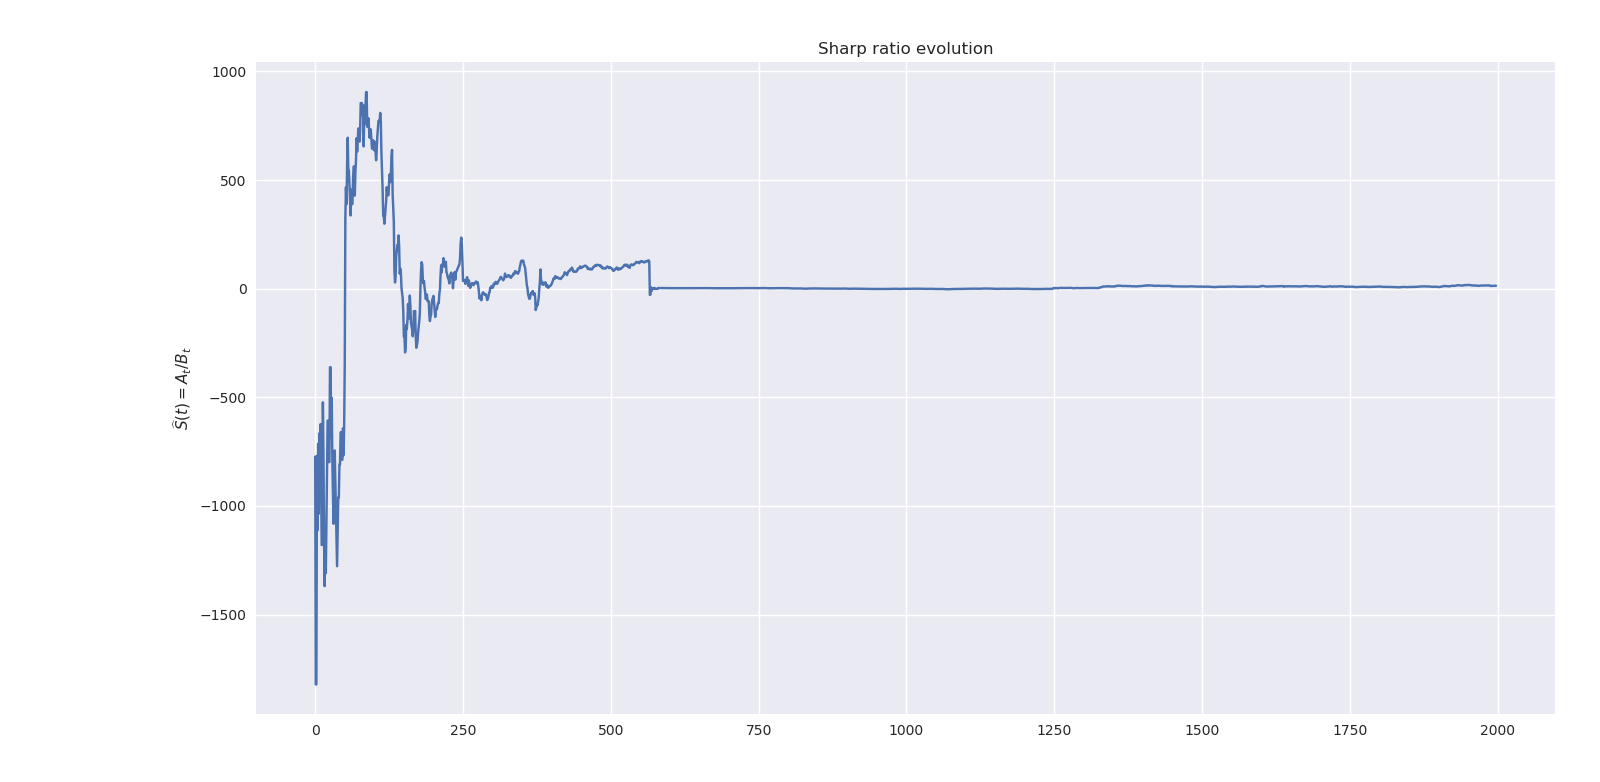
\includegraphics[scale=0.35]{res/Sharpe_ratio_evolution_big}
	\caption{Évolution du \textit{Sharpe ratio} avec $\eta = 0.001$, $A_0 = 0, B_0 = 0$ de $t=0$ à $t=2000$}
\end{figure} 

\begin{figure}[H]
	\centering
	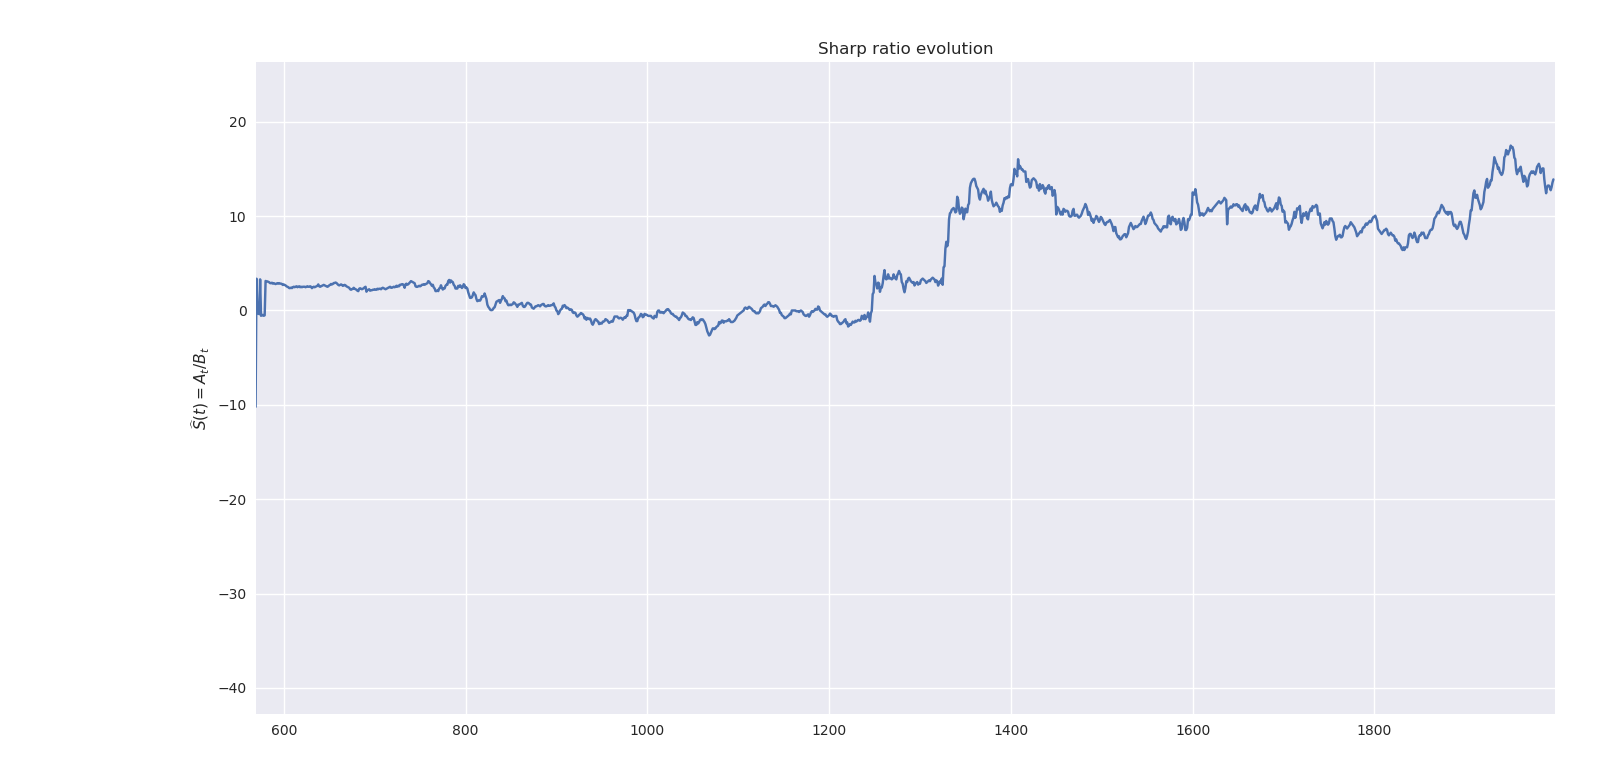
\includegraphics[scale=0.35]{res/Sharpe_ratio_evolution_small}
	\caption{Évolution du \textit{Sharpe ratio} avec $\eta = 0.001$, $A_0 = 0, B_0 = 0$ de $t=0$ à $t=2000$}
\end{figure} 

Nous soulevons également le fait que le \textit{Sharpe ratio} pour des paramètres de bases identiques peut différé d'un lancer à un autre. C'est une conséquence de la corrélation entre le calcul du ratio et la valeur des $w_i$.

\paragraph{}
Afin de voir comment se comportent nos algorithmes sur la durée, nous allons expérimenter avec des paires de monnaies différentes ainsi que sur des périodes de plusieurs années. Cela nous fournira des indications sur la confiance qu'il est possible d'avoir. Notre hypothèse est que sur la longueur il risque d'y avoir des pertes. En effet en se basant sur les mesures plus courtes effectuées précédemment, nous avons soulevé le fait que les gains sont locaux mais ne suffisent pas à compenser les mauvais résultats globaux.

Pour rendre l'ensemble plus lisible et en extraire plus d'informations, une représentation sous forme de tableau a été préférée.
\todo[inline]{Ajouter plot des cours + p\&l pour les trois paires.}

\begin{table}[h!]
	\centering
	\begin{tabular}{|c|c|c|c|c|c|c|}
		\hline
			années & p\&l max & p\&l min & \textit{draw down} & rendement annuel & moyenne & variance\\
			\hline
			2006 & 1.044 & 0.911 & 0.132 & -0.077 & 0.976 & 0.001 \\
			\hline
			2007 & 0.979 & 0.712 & 0.266 & -0.196 & 0.866 & 0.005 \\
			\hline
			2008 & 0.739 & 0.076 & 0.662 & -0.640 & 0.476 & 0.039 \\
			\hline
			2009 & 0.091 & -0.481 & 0.572 & -0.520 & -0.288 & 0.017 \\
			\hline
			2010 & -0.428 & -0.908 & 0.479 & -0.446 & -0.661 & 0.020 \\	
			\hline
	\end{tabular}
\caption{Voici les résultats obtenus pour la paire USD/JPY de 2006 à 2010 avec $|w| = 20$, $2000$ éléments d'entraînement, $500$ de test, une optimisation des
	paramètres toutes les $200$ itérations durant la phase d'apprentissage, $\delta = 0.001, \eta=0.001,\rho=0.01, x = 0.005, y=0.0001$.}
\end{table}

\begin{table}[h!]
	\centering
	\begin{tabular}{|c|c|c|c|c|c|c|}
		\hline
		années & p\&l max & p\&l min & \textit{draw down} & rendement annuel & moyenne & variance\\
		\hline
		2006 & 1.005 & 0.785 & 0.219 & -0.212 & 0.904 & 0.001\\
		\hline
		2007 & 0.805 & 0.703 & 0.102 & -0.058 & 0.753 & 0.001\\
		\hline
		2008 & 0.744 & 0.108 & 0.636 & -0.590 & 0.588 & 0.025\\
		\hline
		2009 & 0.141 & -0.160 & 0.301 & -0.282 & -0.043 & 0.003\\
		\hline
		2010 & -0.077 & -0.218 & 0.140 & -0.018 & -0.150 & 0.001\\
		\hline
	\end{tabular}
\caption{Voici les résultats obtenus pour la paire EUR/USD de 2006 à 2010 avec $|w| = 20$, $2000$ éléments d'entraînement, $500$ de test, une optimisation des
	paramètres toutes les $200$ itérations durant la phase d'apprentissage, $\delta = 0.001, \eta=0.001,\rho=0.01, x = 0.005, y=0.0001$.}
\end{table}

\begin{table}[h!]
	\centering
	\begin{tabular}{|c|c|c|c|c|c|c|}
		\hline
		années & p\&l max & p\&l min & \textit{draw down} & rendement annuel & moyenne & variance\\
		\hline
		2006 & 1.021 & 0.951 & 0.070 & 0.003 & 0.994 & 0.001\\
		\hline
		2007 & 1.006 & 0.881 & 0.124 & -0.078 & 0.936 & 0.001\\
		\hline
		2008 & 0.952 & 0.098 & 0.854 & -0.806 & 0.696 & 0.052\\
		\hline
		2009 & 0.121 & -0.439 & 0.561 & -0.544 & -0.291 & 0.016\\
		\hline
		2010 & -0.426 & -0.973 & 0.546 & -0.533 & -0.628 & 0.017\\
		\hline
	\end{tabular}
	\caption{Voici les résultats obtenus pour la paire GBP/USD de 2006 à 2010 avec $|w| = 20$, $2000$ éléments d'entraînement, $500$ de test, une optimisation des
		paramètres toutes les $200$ itérations durant la phase d'apprentissage, $\delta = 0.001, \eta=0.001,\rho=0.01, x = 0.005, y=0.0001$.}
\end{table}

Les résultats négatifs peuvent sembler impossible mais en précisant certaines choses cela devient possible :
\begin{itemize}
	\item D'un point de vue strictement mathématique, rien n'empêche les valeurs d'être négatives. En ajoutant des \textit{p\&l} négatives à chaque itérations, cela entraîne une décroissance.
	\item Nous utilisons une approximation également présente dans l'article de base \cite{machine_learning_automated_trading}. En calculant les \textit{returns} par $r_i = p_{i} - p_{i-1}$ et en \textit{tradant} exactement une unité à chaque étapes, on obtient une estimation du gain si le profit était réinvesti. En conséquence d'investir exactement une unité de monnaie, cela n'empêche pas les nombres négatifs.
\end{itemize}

Premier élément intéressant, la variance la plus élevée se trouve à chaque fois durant l'année 2008. Cela semble cohérent avec la crise financière de 2008 entraînant ainsi une plus grande volatilité.

De plus, notre hypothèse initiale est vérifié par la moyenne des p\&l. Cette dernière diminue en fil des années, conséquence de la faiblesse du programme sur de longue période.

Concernant les autres mesures, il est difficile d'en apprendre quelque chose excepté le fait que le programme perd de l'argent et que l'année 2008 est la pire de ce point de vue.

Il est intéressant de remarquer que la p\&l maximale de l'année $n+1$ est toujours supérieur à la p\&l minimale de l'année $n$. Cela démontre que malgré la faible capacité de l'algorithme de générer du profit sur le long terme, il reste capable de gagner durant des périodes de temps locales. La piste qui consiste à tenter de généraliser ces gains locaux s'en trouve renforcée.

\paragraph{}
\todo[inline]{Ajouter sur la nécessité de faire plusieurs valeures + intro}
Les graphiques suivants proviennent d'une volonté d'analyser les résultats lorsque l'on fait varier certains paramètres.
\todo[inline]{Ajouter graphique avec fenêtre 1000/250 + fenêtre 4000/1000 sur EUR/USD }
\todo[inline]{Ajouter graphique avec heures -> 2000/500, et jours en 200/50}

\subsubsection{Données}
\todo[inline]{BlaBla sur les données}

\subsubsection{Performances}
\paragraph{}
Le but final est de construire un programme capable d'apprendre et d'effectuer des opérations sur le marché des changes de manière automatique. Il convient de s'intéresser à la performance. En effet, même dans le cas où un algorithme serait capable de trouver la bonne direction à 100\%, si cette opération était trop lente cela ne servirait à rien. Nous allons donc réaliser plusieurs mesures dans le but de découvrir les périodes possible de \textit{trading}.

\paragraph{}
Sachant qu'une étape de \textit{backtesting} consiste à apprendre avec 2000 éléments et de prédire les 500 éléments suivants, pour 100 itérations, le programme prend en moyenne 11s\footnote{La moyenne porte sur 100 essais différents afin d'avoir un résultat stable.}.

D'après cette mesure,  nous pouvons d'utiliser ce programme pour du \textit{trading} de l'ordre de la minute. Qu'en est-t-il d'un temps plus court ?

Avec des mesures plus précises sur les sous-parties du programme, nous obtenons, pour 1000 entraînements avec 2000 éléments, 0.12s en moyenne. On peut considérer que la partie de test est négligeable, car le calcul, à partir des poids est très simple. Ceci est confirmé par le fait qu'il a été impossible d'obtenir un temps avec la fonction \lstinline|System.currentTimeMillis()|, l'exécution est donc souvent plus courte qu'une milliseconde.
Nous pouvons donc envisager de faire des opérations chaque seconde.

\paragraph{}
Sur les 0.12s en moyenne, il est intéressant de savoir quelle partie coûte le plus en terme de calcul.
Pour les mêmes paramètres que précédemment, nous avons :
\begin{itemize}
	\item La mise à jour des poids prend $83\mu$s.
	\item Le calcul du signal prend $25.5\mu$s\footnote{Cela confirme que le calcul du signal est négligeable dans le cadre d'un \textit{trading} d'une seconde.}.
	\item La mise à jour des paramètres\footnote{La mise à jour s'effectue une fois toute les 200 étapes durant une étape d'entraînement.} prend $220\mu$s.
\end{itemize}

Il apparaît que l'optimisation des paramètres est l'étape la plus coûteuse. Si l'on réduit le nombre d'étapes nécessaires à 2 afin d'obtenir un cas extrême, le temps devient $2139\mu$s. Cela représente un facteur 10.

Il est donc possible en utilisant des valeurs adéquates pour les paramètres, d'utiliser ce logiciel avec une granularité d'une seconde.

Ces performances sont le résultat de plusieurs améliorations algorithmiques. En effet, lors des premières versions, le code réalisait les itérations initiales rapidement puis le temps augmentait. Cela peut sembler étonnant surtout pour du code tournant sur une JVM, qui optimise le bytecode mieux qu'un programmeur. Le soucis venait de la quantité d'information stocké. Initialement, les informations utiles aux calculs, comme le \textit{return}, le \textit{p\&l} précédent et autres étaient stockés dans un vecteur, qui au fil des itérations croissait. La conséquence fut que le vecteur devant plus lourd en mémoire, prenait également plus de temps à être manipulé, augmentant ainsi le temps global.

Afin de corriger cela, nous n'avons gardé que le minimum d'informations utiles, ce qui correspondaient souvent à certains nombres de l'itérations $n-1$. La mise à jour de ces valeurs se fait donc à chacun fin de boucle rendant le temps de calcul linéaire au nombre d'étapes de \textit{backtesting}.
 
\subsection{Conclusion}
\paragraph{}
Comme mentionné dans l'introduction, le but de ce projet était d'implémenter l'algorithme, de le faire fonctionner, de le tester et de trouver des pistes
d'amélioration.

L'implémentation a été compliquée à cause du manque d'information dans l'article. L'algorithme n'y est que très peu décrit et, mis à part certaines 
équations, il n'y a aucun pseudo-code pour le comprendre. Il s'agît juste de descriptions vagues sur le fonctionnement et l'idée du programme. À partir de
cela, nous avons dû grandement interpréter et nous baser sur d'autres recherches théoriques afin de combler les manques. Il nous a fallu faire des compromis
afin de faire fonctionner le programme, ce qui explique les divergences rencontrées avec l'idée initiale.

Ces divergences peuvent être prises comme des améliorations. En effet, l'implémentation initiale ne marchait pas et c'est grâce à ces idées que nous avons
réussi à obtenir des résultats. Nous pensons principalement aux variantes de la descente du gradient qui ont permises de diminuer les risques de
\texttt{NaN}.

\paragraph{}
En terme de résultats, contrairement à l'article, nous avons effectué nos mesures sur plusieurs cours à des périodes différentes. Un des gros problèmes
provient des différences entre deux \textit{runs}. Il est compliqué de dire si l'algorithme est performant ou non, car cela varie énormément. De plus,
l'optimisation et la recherche de solutions sont ardues à cause de ce phénomène. Il nous est impossible de dire après un bon profit si cela est du à la
chance ou non, et réciproquement avec les mauvais résultats.

On peut noter que malgré cela, l'algorithme trouve toujours le moyen de faire des profits indépendamment de la tendance ou des résultats précédant, ce
qui est une satisfaction. En effet, ce phénomène implique qu'il y a effectivement apprentissage et que le réseau est capables sous certaines conditions
de réussir à produire et interpréter un signal correctement. Afin
d'améliorer le programme, il faudrait comprendre ce qui provoquer ces profits locaux et le généraliser afin d'obtenir un profit cumulé global croissant, ce qui
n'est pas forcément le cas actuellement. En comprenant, le phénomène local de ce gain, on pourrait changer l'approche de l'algorithme et en accroître les
performances.

En fixant les métas-paramètres\footnote{À cause du problème soulevé dans la section \textit{Layer 3}}, le \textit{stop trailing loss} est moins visible
que sur d'autres exemples. Ce qui nous permet de mentionner un problème récurrent dans ce projet : de part le manque d'information, les valeurs initiales
de tout les paramètres sont extrêmement difficiles à trouver. La moindre petite variation peut aboutir à un crash ou à un profit \texttt{NaN}. Le caractère
empirique du domaine de l'optimisation et du \textit{machine learning}, ne nous permet pas d'avoir des valeurs standards fonctionnant avec n'importe quel
algorithme. Cela revient donc à tester plusieurs valeurs en espérant qu'une fonctionnera.

\paragraph{}
Concernant la question de recherche, nous n'avons pas été capable de faire fonctionner l'idée originale. Cependant nous avons pu saisir les raisons ou 
éléments qui empêchaient son fonctionnement. Nous avons ensuite proposer des améliorations reposant sur ces constations. Ces dernières ont permis 
d'améliorer les performances de l'algorithme tout en reposant sur des bases mathématiques solides.

\paragraph{}
Concernant les pistes pour des recherches futures, nous en voyons plusieurs :
\begin{itemize}
 \item Améliorer les métas-paramètres.
 \item Intégrer une version alternative de la descente du gradient.
 \item Proposer un réseau multi-couche.
\end{itemize}

Pour les métas-paramètres, il a plusieurs points à soulever. Il faudrait dans un premier temps trouver les domaines des valeurs afin de permettre
une recherche de l'optimum plus aisée. De plus, si nous pouvions réduire le nombre de métas-paramètres, comme nous l'avons fait pour $\rho$ avec l'algorithme
RMSProp, cela permettrait d'améliorer la vitesse tout en proposant des méthodes d'optimisation plus précises et donc d'augmenter la performance global.

En utilisant, une version alternative de la descente du gradient, comme le RMSProp, le Adagrad ou le Adadelta, nous pourrions éviter certain soucis
inhérent à la descente du gradient. Cette dernière est une méthode ancienne et toutes celles proposées sont des améliorations qui tendent à pallier les
problèmes de la descente du gradient. De plus, cela pourrait avoir des effets bénéfiques sur l'ensemble du programme en diminuant le nombre de paramètres
et donc la complexité interne de l'algorithme, sans faire de concession en terme de performances.

La construction d'un réseau de neurones n'est pas une science exacte. Cependant, le fait d'ajouter une ou plusieurs couches permettrait d'augmenter la 
vitesse d'apprentissage de ce dernier et de diminuer les erreurs. En sacrifiant du temps de calcul, car un réseau de neurones à plusieurs couches est plus
lent qu'un autre à une seule couche, on pourrait deviner la direction plus aisément. De plus avec les gains de vitesse des propositions précédentes, les
performances resteront bonnes.

%%%%%%%%%%%%%%%%%%%%%%%%%%%%%%%%%%%%%%%%%%%%%%%%%%%%%%%%%%%%%%%%%%%%%%%%%%
% début de la bibliographie %%%%%%%%%%%%%%%%%%%%%%%%%%%%%%%%%%%%%%%%%%%%%%
%%%%%%%%%%%%%%%%%%%%%%%%%%%%%%%%%%%%%%%%%%%%%%%%%%%%%%%%%%%%%%%%%%%%%%%%%%
\newpage
\bibliographystyle{plain}
\nocite{*}
\bibliography{bibliographie}


\end{document}
